% DISCELL -- RECOMB submission, supplement (separate PDF).
% Sections are numbered S1, S2, ...; figures, tables and equations S1, S2, ...
% Main-text labels are imported from main.aux via xr-hyper (no prefix).
\documentclass[letterpaper,10pt]{article}

\usepackage[letterpaper,margin=1in]{geometry}

\usepackage[numbers,sort&compress]{natbib}
\usepackage{amsmath,amssymb,amsthm,bm,mathtools}
\usepackage{graphicx}
\usepackage{booktabs,multirow,array,longtable}
\usepackage{subcaption}
\usepackage{xcolor}
\usepackage{microtype}
\usepackage{enumitem}
% floats stay in their own section (no tables flushed after the bibliography)
\usepackage[section]{placeins}
\renewcommand{\topfraction}{0.9}
\renewcommand{\bottomfraction}{0.8}
\renewcommand{\textfraction}{0.07}
\renewcommand{\floatpagefraction}{0.75}
\setcounter{topnumber}{4}
\setcounter{bottomnumber}{2}
\setcounter{totalnumber}{6}
\PassOptionsToPackage{hyphens}{url}
\usepackage{xr-hyper}
\usepackage[colorlinks=true,linkcolor=blue!60!black,citecolor=blue!60!black,urlcolor=blue!60!black]{hyperref}
\usepackage[capitalise]{cleveref}
% short reference names to save space (author, 2026-10-01)
\crefname{figure}{Fig.}{Figs.}\Crefname{figure}{Fig.}{Figs.}
\crefname{table}{Table}{Tables}\Crefname{table}{Table}{Tables}
\crefname{section}{Sec.}{Secs.}\Crefname{section}{Sec.}{Secs.}
\crefname{equation}{Eq.}{Eqs.}\Crefname{equation}{Eq.}{Eqs.}
\renewcommand{\figurename}{Fig.}

\graphicspath{{../aistats/figures/}}
\newcommand{\tablesdir}{../aistats/tables/generated}
% ---------------------------------------------------------------------------
% Notation and editorial macros for the DISCELL manuscript (RECOMB copy of ../aistats/macros.tex)
% ---------------------------------------------------------------------------
\newcommand{\needsource}{\textcolor{red}{\textbf{[NEEDS A SOURCE]}}}
\newcommand{\todo}[1]{\textcolor{orange}{\textbf{[TODO: #1]}}}
\newcommand{\pending}[1]{\textcolor{violet}{\textbf{[PENDING RUNS: #1]}}}
% editorial flags and reading-order markers: no-ops in the RECOMB version
% (kept so that text copied from the AISTATS sources compiles; delete calls when editing)
\DeclareRobustCommand{\flag}[2]{\ignorespaces}
\DeclareRobustCommand{\readorder}[1]{\ignorespaces}
% code link placeholder (the clean repository comes later)
\newcommand{\codelink}{\textcolor{violet}{\texttt{[URL to be added]}}}

% vocabulary of the generated tables (shared by both manuscripts): RECOMB words (STYLE.md); ../aistats/macros.tex defines the AISTATS ones
\newcommand{\termSpill}{spill-over}
\newcommand{\TermSpill}{Spill-over}
\newcommand{\termSpillFrac}{spill-over fraction}
\newcommand{\TermSpillFrac}{Spill-over fraction}
\newcommand{\termReloc}{relocation}
\newcommand{\TermReloc}{Relocation}
\newcommand{\termInflux}{spill-over influx}
\newcommand{\TermInflux}{Spill-over influx}

% operators
\DeclareMathOperator{\sgop}{sg}
\newcommand{\sg}[1]{\sgop\!\left[#1\right]}
\DeclareMathOperator{\KL}{KL}
\DeclareMathOperator{\softmax}{softmax}
\DeclareMathOperator{\Mult}{Multinomial}
\DeclareMathOperator{\Pois}{Poisson}
\DeclareMathOperator{\CE}{CE}
\DeclareMathOperator{\diag}{diag}
\DeclareMathOperator{\logdet}{logdet}
\DeclareMathOperator{\embed}{embed}
\DeclareMathOperator{\onehot}{onehot}
\DeclareMathOperator{\GAT}{GATv2}
\DeclareMathOperator{\I}{I}
\DeclareMathOperator{\E}{\mathbb{E}}
\DeclareMathOperator{\Var}{Var}
\DeclareMathOperator{\corr}{corr}
\DeclareMathOperator{\NMI}{NMI}
\DeclareMathOperator{\simop}{sim}
\newcommand{\att}{\pi}   % attention weight, distinct from the loss weights alpha

% sets and fields
\newcommand{\R}{\mathbb{R}}
\newcommand{\Nat}{\mathbb{N}}
\newcommand{\N}{\mathcal{N}}
\newcommand{\simplex}[1]{\Delta^{#1}}
\newcommand{\nbr}[1]{\mathcal{N}_{#1}}

% vectors
\newcommand{\vx}{\mathbf{x}}
\newcommand{\vy}{\mathbf{y}}
\newcommand{\vz}{\mathbf{z}}
\newcommand{\vw}{\mathbf{w}}
\newcommand{\vc}{\mathbf{c}}
\newcommand{\vv}{\mathbf{v}}
\newcommand{\vu}{\mathbf{u}}
\newcommand{\vB}{\mathbf{B}}
\newcommand{\vI}{\mathbf{I}}
\newcommand{\vPhi}{\boldsymbol{\Phi}}
\newcommand{\vrho}{\boldsymbol{\rho}}
\newcommand{\rhobar}{\bar{\boldsymbol{\rho}}}
\newcommand{\vp}{\mathbf{p}}
\newcommand{\vmu}{\boldsymbol{\mu}}
\newcommand{\vsigma}{\boldsymbol{\sigma}}
\newcommand{\wbreve}{\breve{\mathbf{w}}}
\newcommand{\ybar}{\bar{\mathbf{y}}}
\newcommand{\Phibar}{\bar{\boldsymbol{\Phi}}}
\newcommand{\Sig}{\boldsymbol{\Sigma}}
\newcommand{\Sighat}{\hat{\boldsymbol{\Sigma}}}
\newcommand{\lbar}{\bar{\ell}}
\newcommand{\ephi}{e^{\Phi}}
\newcommand{\Ephi}{E_{\Phi}}
\newcommand{\dz}{d_z}
\newcommand{\dw}{d_w}
\newcommand{\dPhi}{d_{\Phi}}
\newcommand{\alphaz}{\alpha_z}
\newcommand{\alphaw}{\alpha_w}
\newcommand{\alphaa}{\alpha_a}
\newcommand{\mpsi}{m_{\psi}}
\newcommand{\Pen}{\mathrm{Pen}}
\newcommand{\Adv}{\mathrm{Adv}}
\newcommand{\dCE}{\Delta\!\CE}
\newcommand{\um}{\,\mu\text{m}}

\newtheorem{proposition}{Proposition}
\newtheorem{remark}{Remark}
\theoremstyle{definition}
\newtheorem{definition}{Definition}

% main-text captions imported through xr may use \suppref; inside the supplement it reads "Section S3"
\newcommand{\suppref}[1]{Section~\ref{#1}}

\externaldocument[][nocite]{main}[main.pdf]   % labels only: each document keeps its own bibliography numbers

\renewcommand{\thesection}{S\arabic{section}}
\renewcommand{\thefigure}{S\arabic{figure}}
\renewcommand{\thetable}{S\arabic{table}}
\renewcommand{\theequation}{S\arabic{equation}}
\renewcommand{\theHsection}{S\arabic{section}}
\renewcommand{\theHfigure}{S\arabic{figure}}
\renewcommand{\theHtable}{S\arabic{table}}
\renewcommand{\theHequation}{S\arabic{equation}}

\title{DISCELL: Supplementary Material}
\author{}
\date{}

\begin{document}
\maketitle

% Guide for the reviewer: where each claim of the main text is checked (not a float, so it takes no table number)
\section*{Guide}
Sections follow the main text: \cref{app:derivations,app:implementation} back \cref{sec:method}, \cref{app:experimental,app:readouts-section} \cref{sec:setup}, \cref{app:simulation} \cref{sec:simulation}, \cref{app:full-results} \crefrange{sec:intrinsic-response}{sec:relocation}, \cref{app:sensitivity-section} \cref{sec:results-sweep}, and \cref{app:limitations} collects the limitations.

\begin{center}
\footnotesize
\setlength{\tabcolsep}{4pt}
\begin{tabular}{@{}p{0.36\textwidth}p{0.17\textwidth}p{0.4\textwidth}@{}}
\toprule
Claim & Main text & Check in the supplement \\
\midrule
Model, objective, bound on $\kappa$ & \cref{sec:method} & \cref{app:derivations}, proof \cref{app:kappa}, symmetries \cref{app:symmetries}; settings \cref{app:architecture}, calibration \cref{app:S-calibration} \\
C1 Spill-over is bounded, not estimated; breakdown points & \cref{sec:sweep,sec:results-sweep}, \cref{tab:kappa-star} & \cref{app:sweep}: \cref{tab:S-contrasts}, \cref{fig:breakdown-data}, \cref{tab:breakdown-traj}; \cref{app:S-planted-spillover}; \cref{app:sensitivity} \\
C2 Less residual niche signal, more intrinsic state & \cref{sec:comparison}, \cref{fig:tradeoff} & \cref{tab:probe}, \cref{tab:battery}; methods \cref{app:baselines} \\
C3 $\vz$ keeps type and cycle & \cref{sec:results-z} & \cref{tab:headline-full}, \cref{tab:probe}; definitions \cref{app:readouts} \\
C4 $\vw$ carries the niche; sublabels split & \cref{sec:results-w} & \cref{app:response}, \cref{app:moran}, \cref{app:subtype}; limits \cref{app:planted-percell}, \cref{app:recon-modes} \\
C4b Response programmes & \cref{sec:programmes} & \cref{fig:hallmarks}, \cref{app:response} \\
C5 Relocation & \cref{sec:relocation} & \cref{app:readouts}, \cref{tab:cellina-cf}, \cref{tab:transport-heldout} \\
C6 Reconstruction and speed & \cref{sec:comparison} & \cref{tab:battery}, \cref{tab:timing} \\
C7 Simulation & \cref{sec:simulation} & \cref{app:synthetic}, \cref{tab:synthetic}, \cref{fig:synthetic-misspec}, \cref{app:planted} \\
Data and fairness & \cref{sec:setup} & \cref{app:sections}, \cref{app:baselines}; limitations \cref{app:limitations} \\
\bottomrule
\end{tabular}
\end{center}

% order follows the main text: model (S1-S2), data and readouts (S3-S4), simulation (S5), tissue results (S6), sweep (S7), limitations (S8)
% S1: copied from ../aistats/appendix (see SETUP_REPORT.md for provenance); edit here, not there.
% Trimmed 2026-10-01 (agent A): notation table added; proof of Prop. 1 moved here from S2;
% closed-form penalty, amplification heuristic and learned-variance discussion cut (history).
\section{Model: Notation, Derivations and Proofs}
\label{app:derivations}

\begin{table}[!htbp]
\centering
\caption{Notation.}
\label{tab:S-notation}
\small
\begin{tabular}{@{}lp{0.78\textwidth}@{}}
\toprule
Symbol & Meaning \\
\midrule
$\vx_i$, $\ell_i$ & count vector of cell $i$ over $G$ genes; its total, conditioned on and never modelled; $\lbar$ the section's median total \\
$t_i \in \{1,\dots,K\}$ & lineage label \\
$\vz_i \in \R^{\dz}$ & intrinsic state; prior $\N(\mathbf{0},\vI)$ \\
$\vw_i \in \R^{\dw}$ & response; prior $\N(\mpsi(\vc_i,t_i), \sigma_w^2\vI)$, $\sigma_w = 1$ \\
$\vc_i$ & niche descriptor: attention over the neighbours' types $\oplus$ masked image embedding $\vPhi_i$ $\oplus$ isolation flag \\
$\vy_i$, $\vPhi_i$ & neighbour-type composition; image embedding with a disc over the cell set to zero \\
$\vrho_i$ & clean composition $\softmax(a(\vz_i) + \vB\vw_i)$; $a$ the decoder, $\vB \in \R^{G\times\dw}$ the loadings \\
$\nbr{i}$, $\beta_{ij}$ & neighbour set in the pruned Delaunay graph; fixed spill-over kernel \\
$\rhobar_i$ & spill-over influx $\sum_{j\in\nbr{i}}\beta_{ij}\vrho_j$ \\
$\kappa$, $\vp_i$ & spill-over fraction, fixed per fit and swept; fitted composition $(1-\kappa)\vrho_i + \kappa\rhobar_i$ \\
$\bar\kappa_i$ & largest spill-over fraction compatible with cell $i$'s composition (\cref{prop:kappa-bound}) \\
$\vmu_{z,i}$, $\vmu_{w,i}$ & posterior means, which the probes and readouts use \\
$\alphaz$, $\alphaw$, $\alphaa$, $\omega$ & weights of the $\vz$-divergence, the $\vw$-divergence, the adversary and the intrinsic path \\
\bottomrule
\end{tabular}
\end{table}

\subsection{The Reconstruction Bound}
\label{app:bound}

Fix a cell $i$ and hold $\vc_i$ and $\rhobar_i$ constant, as \cref{sec:batching} does (we suppress the conditioning on $\rhobar_i$). Under the variational family $q(\vz)\,q(\vw \mid \vc_i, t_i, \vz, \vx_i)$, Jensen's inequality gives
\begin{equation}
  \log p(\vx_i \mid \vc_i, t_i)
  \geq \E_{q(\vz)}\Big[\E_{q(\vw \mid \vz)}\big[\log p(\vx_i \mid \vz, \vw)\big] - \KL\big(q(\vw \mid \vz)\,\|\,p(\vw \mid \vc_i, t_i)\big)\Big] - \KL\big(q(\vz)\,\|\,p(\vz)\big) =: L_i.
  \label{eq:jensen}
\end{equation}
Because $q(\vw \mid \cdot)$ conditions on the sampled $\vz$, the $\vw$-divergence sits inside $\E_{q(\vz)}$; evaluating the closed-form Gaussian divergence at the single reparameterised draw of $\vz$ is an unbiased one-sample estimate. Summed over cells, with each neighbour's latents drawn from its own posterior (\cref{app:tiles}), $\sum_i L_i$ estimates the evidence lower bound of the coupled model under a fully factorised family. The per-cell bounds are not independent, since $\rhobar_i$ depends on the neighbours' latents; the stop-gradient removes the cross terms from the gradient, so training is a fixed-point iteration in which each step treats the current $\rhobar$ as data.

\paragraph{Isolated cells.} For a cell with no neighbours after pruning, $\rhobar_i = \mathbf{0}$ and the mixture of \cref{eq:gen-p} would sum to $1-\kappa$, charging the cell for spill-over it cannot receive. The mixture is therefore renormalised per row,
\begin{equation}
  \vp_i = \frac{(1-\kappa)\,\vrho_i + \kappa\,\rhobar_i}{(1-\kappa) + \kappa\sum_{j \in \nbr{i}}\beta_{ij}},
  \label{eq:S-renorm}
\end{equation}
so that an isolated cell has $\vp_i = \vrho_i$; for connected cells the denominator is one. Probabilities are floored at $10^{-8}$ inside the logarithm. The graph part of an isolated cell's niche descriptor is set to zero and its isolation flag raised; the image part stays. Isolated cells are left out of the type-mean targets $\ybar(t)$ and $\Phibar(t)$ but not out of the adversary or the probes.

\paragraph{Why a multinomial.} Independent Poisson counts, conditioned on their total $\ell_i$, are multinomial; since $\ell_i$ is observed, the multinomial needs no library-size latent and does not count depth twice. The mixture of \cref{eq:gen-p} is exact if the cell's own and the spill-over transcripts are independent Poisson sources and the spill-over rate scales with the receiving cell's own rate (\cref{app:limitations}). Negative-binomial sources are not closed under addition, and a dispersion on the mixed counts would absorb part of what the mixture should explain. At a median of $178$ to $1{,}401$ counts per cell over five thousand genes (\cref{tab:sections}), gene-wise overdispersion cannot be estimated in any case; the natural extension is a Dirichlet-multinomial with one concentration scalar.

\subsection{The Intrinsic Path and the Status of the Objective}
\label{app:pathb}
\label{app:posterior-reg}

Restricting the variational family to $q(\vw) := p(\vw \mid \vc_i, t_i)$ gives a second bound on the same evidence,
\begin{equation*}
  \log p(\vx_i \mid \vc_i, t_i) \geq \E_{q(\vz)}\E_{p(\vw \mid \vc_i, t_i)}\big[\log p(\vx_i \mid \vz, \vw)\big] - \KL\big(q(\vz)\,\|\,p(\vz)\big) =: L_i^{z}.
\end{equation*}
Each bound carries its own $\vz$-divergence, so $L_i + \omega L_i^{z} \le (1+\omega)\log p(\vx_i \mid \vc_i, t_i)$ contains $-(1+\omega)\KL(q(\vz_i)\|p(\vz_i))$, with gap $\KL\big(q(\vz)q(\vw \mid \vz)\,\|\,p(\vz,\vw \mid \cdot)\big) + \omega\,\KL\big(q(\vz)p(\vw \mid \vc_i,t_i)\,\|\,p(\vz,\vw \mid \cdot)\big)$. This mirrors the two-bound objective of \citet{slavutsky2025}, except that both of our terms bound the same evidence. One $q(\vz)$ serves two families, so its optimum is a compromise. The path is the only term that rewards $\vz$ for being informative, since the prior on $\vw$ never references $\vz$; it decodes through the same spill-over mixture at the same $\kappa$. At the final configuration it acts on the allocation: without it, $\vw$ takes up type signal (\cref{app:sensitivity}).

\paragraph{Scaling of the weights.} The reconstruction terms of \cref{eq:objective} are divided by $\ell_i$, so that weights transfer between sections of different depth; reconstruction becomes $O(1)$ while the divergences stay absolute. At $\alphaz = \alphaw = 1/\lbar$ and $\alphaa = 0$, $J$ is proportional to $L_i + \omega L_i^{z}$ for a cell of median depth, and that point is the reference for the weights; $\alphaz = \tfrac12/\lbar$ restores a single charge of the $\vz$-divergence at $\omega = 1$. The response weight departs from it deliberately ($\alphaw = 0.1$; \cref{app:S-calibration}). At that weight the response posterior stays close to its prior mean, so the response readouts are in effect readouts of the context regression $\mpsi(\vc_i, t_i)$, with exceptions in subtype recovery (\cref{app:subtype}); a planted per-cell response is not detected at this weight (\cref{app:planted-percell}). The per-cell scaling also weights a cell's divergences, relative to its own bound, in proportion to its depth (\cref{app:kl-maps}), the price of transferable weights.

\paragraph{Status of the objective.} Once a weight departs from $1/\lbar$, $J$ is a weighted surrogate rather than a bound. Neighbour compositions enter under a stop-gradient and, with the adversary, the fit is a saddle point of a two-player game, so training does not maximise $J$ as a single function. The invariance term is part of no bound: it is posterior regularisation \citep{ganchev2010}, a constraint $\I(\vz; [\vy, \vPhi] \mid t) = 0$ on the aggregate of the encoder's outputs, the status \citet{slavutsky2025} give their adversarial term; the generative model does not model $\vy$ or $\vPhi$. We therefore claim no likelihood-based uncertainty for $q$: the reported variability comes from the spill-over sweep and the seeds. $\kappa$ is not a hyperparameter but the sweep axis.

\subsection{The Spill-over Fraction: Proof of Proposition~1 and the Grid}
\label{app:kappa}

\begin{proof}[Proof of \cref{prop:kappa-bound}]
The clean composition implied by $\kappa'$ is $\vrho_i(\kappa') = (\vp_i - \kappa'\rhobar_i)/(1-\kappa')$, which sums to one for every $\kappa'$ and is non-negative in gene $g$ if and only if $\kappa'\bar\rho_{ig} \le p_{ig}$; this holds for every gene if and only if $\kappa' \le \bar\kappa_i$. Since $p_{ig}/\bar\rho_{ig} = \kappa + (1-\kappa)\rho_{ig}/\bar\rho_{ig} \ge \kappa$, the true value lies below the bound, and meets it exactly when a gene the neighbours express has zero share in the cell's own composition.
\end{proof}

A section-wide $\kappa$ must respect the bound of every cell, and the data pin it only through a gene the cell cannot express itself or through a second view of the cell. With counts the bound is soft, since a $\kappa$ above it charges a cell for neighbour transcripts it does not show. The bound holds with the neighbours' clean profiles fixed and is not computed on our sections, so a contrast that survives the grid is shown to survive spill-over fractions up to $0.4$, not every fraction the data allow. The grid runs from zero, the nested no-correction null, to $0.4$: a typical cell on this platform carries misassigned transcripts of about a tenth of its counts \citep{yang2025mistic}, which the operating point $0.1$ matches and the top of the grid exceeds several times. Estimating $\kappa$ would need two views of one cell at different spill-over levels, such as a nuclear/extranuclear split of the transcripts, with a multinomial over $2G$ bins; we leave it as future work.

\subsection{Symmetries of the Response}
\label{app:symmetries}

Given $\kappa$, the response coordinates carry at least the symmetries of \cref{prop:S-symmetries}; we do not show that there are no others. The statement treats $a$, $\mpsi$ and the posterior networks as arbitrary functions of their inputs, each map is applied to every cell at once, and the response posterior is $\N(\vmu_{w,i}, \diag\boldsymbol{\nu}_{w,i}^2)$.

\begin{proposition}[Symmetries of the response]\label{prop:S-symmetries}
Fix $\kappa$, the graph and the kernel.
\begin{enumerate}[label=(\alph*), leftmargin=*, nosep]
\item \emph{Rotation.} For orthogonal $\mathbf{Q} \in \R^{\dw \times \dw}$, the map $\vw_i \mapsto \mathbf{Q}\vw_i$, $\vB \mapsto \vB\mathbf{Q}^\top$, $\mpsi \mapsto \mathbf{Q}\mpsi$ leaves the distribution of the counts in \cref{eq:gen-z,eq:gen-w,eq:gen-rho,eq:gen-rhobar,eq:gen-p,eq:gen-x} unchanged, and, with each posterior mapped to $\N(\mathbf{Q}\vmu_{w,i},\, \mathbf{Q}\diag\boldsymbol{\nu}_{w,i}^2\mathbf{Q}^\top)$, every term of the objective $J$ of \cref{eq:objective}. The mapped posterior is again diagonal, so $J$ is unchanged within the diagonal family, when $\mathbf{Q}$ is a signed permutation.
\item \emph{Constants over genes.} For any scalar function $c(\vz)$ and any $\mathbf{b} \in \R^{\dw}$, the map $a \mapsto a + c\,\mathbf{1}$, $\vB \mapsto \vB + \mathbf{1}\mathbf{b}^\top$ leaves every clean composition, and hence $J$, unchanged.
\item \emph{Per-type translation.} Suppose there is a function $\tau$ with $\tau(\vz) = t_i$ for every $\vz$ in the support of $q(\vz_i)$, for every cell $i$. For any $\boldsymbol{\delta}_1, \dots, \boldsymbol{\delta}_K \in \R^{\dw}$, the map $\vw_i \mapsto \vw_i + \boldsymbol{\delta}_{t_i}$ (the posterior mean with it), $\mpsi(\vc, t) \mapsto \mpsi(\vc, t) + \boldsymbol{\delta}_t$, $a(\vz) \mapsto a(\vz) - \vB\boldsymbol{\delta}_{\tau(\vz)}$ leaves $J$ unchanged.
\end{enumerate}
A rescaling $\vw \mapsto \mathbf{S}\vw$, $\vB \mapsto \vB\mathbf{S}^{-1}$ with $\mathbf{S}$ diagonal and some $|S_{kk}| \neq 1$ is not a symmetry, because it changes the prior divergence.
The centred shift $\vB(\vw_i - \bar\vw_t)$, with $\bar\vw_t$ the mean response of type $t$, and the realised prior shift $\vB[\mpsi(\vc_i, t_i) - \mpsi(\bar\vc_t, t_i)]$, with $\bar\vc_t$ its mean niche descriptor, each centred over genes, are unchanged by all three maps.
\end{proposition}

\noindent The fixed prior scale $\sigma_w$ is what removes the rescaling: a learned constant $\sigma_w$ would absorb it, and a learned conditional $\sigma_w(\vc, t)$ could shrink the divergence by inflating the prior wherever it bites. Loadings are read only after centring each column over genes. The per-type translation holds only approximately, because the decoder sees $\vz$ but not $t$ and posteriors of different types overlap; it is a near-flat direction that the optimisation, not the likelihood, decides. Hence the magnitude $\|\vw_i\|$, and any ranking of types by it, is a statement about the gauge; the gauge-free quantities are the two centred shifts. A ``clean'' per-cell profile must be decoded at a reference niche such as $\bar\vc_t$, not at $\vw = \mathbf{0}$, which would subtract the type offset along with the niche effect. Differences between two niches, which the relocation reads, are gauge-free. The allocation between $\vz$ and $\vw$ rests on the conditional invariance, the intrinsic path and $\dw < \dz$. For $\vw$ given the niche this is in the spirit of the auxiliary-variable setting of \citet{khemakhem2020}, whose guarantee we do not establish for this likelihood; for $\vz$ no comparable guarantee exists without the constraint \citep{locatello2019}, which the held-out probe verifies rather than assumes.

\begin{proof}[Proof of \cref{prop:S-symmetries}]
Write $\mathbf{u}_i = a(\vz_i) + \vB\vw_i$ for the logits of \cref{eq:gen-rho}. The terms of $J$ that involve $a$, $\vB$, $\vw$ or $\mpsi$ are the two reconstruction terms, which are expectations of functions of the logits of cell $i$ and, through $\rhobar_i$, of its neighbours, and the prior divergence of $\vw$. The $\vz$-divergence and the invariance term depend only on $q(\vz_i)$ and $t_i$ and are untouched by all three maps.

(a) $\vB\mathbf{Q}^\top\mathbf{Q}\vw_i = \vB\vw_i$, so every draw has the same logits, hence the same $\vrho_i$, $\rhobar_i$ and $\vp_i$. Under the prior of \cref{eq:gen-w}, $\mathbf{Q}\vw_i \sim \N(\mathbf{Q}\mpsi, \sigma_w^2\mathbf{Q}\mathbf{Q}^\top) = \N(\mathbf{Q}\mpsi, \sigma_w^2\vI)$, which is the mapped prior, so the distribution of the counts is unchanged. In $J$, the mapped posterior and the mapped prior are the images of the originals under $\vw \mapsto \mathbf{Q}\vw$, so both reconstruction terms, the second of which draws $\wbreve_i$ from the prior, are unchanged, and the divergence between two distributions is invariant under a common bijection. For a signed permutation, $\mathbf{Q}\diag\boldsymbol{\nu}^2\mathbf{Q}^\top$ is the diagonal matrix with the entries of $\boldsymbol{\nu}^2$ permuted.

(b) The logits become $\mathbf{u}_i + \big(c(\vz_i) + \mathbf{b}^\top\vw_i\big)\mathbf{1}$, a shift by a scalar that is the same for every gene, and the softmax is invariant under such a shift. Every clean composition is therefore unchanged for every draw, and no other term of $J$ involves $a$ or $\vB$.

(c) For $\vz$ in the support of $q(\vz_i)$, $\tau(\vz) = t_i$, so the logits become $a(\vz) - \vB\boldsymbol{\delta}_{t_i} + \vB(\vw + \boldsymbol{\delta}_{t_i}) = a(\vz) + \vB\vw$, both for posterior draws, which are shifted with the posterior mean, and for prior draws $\wbreve_i$, which are shifted with $\mpsi$. The same holds for every neighbour, so $\rhobar_i$ is unchanged. The divergence between two Gaussians with the same covariances depends on their means only through their difference, and both means are shifted by $\boldsymbol{\delta}_{t_i}$.

Rescaling. With $\lambda_k = S_{kk}^2$, dimension $k$ of the divergence between $\N(\vmu_{w,i}, \diag\boldsymbol{\nu}_{w,i}^2)$ and $\N(\mpsi, \sigma_w^2\vI)$ changes under the map by $\tfrac12\big[(\lambda_k - 1)A_{ik} - \log\lambda_k\big]$ with $A_{ik} = \big(\nu_{w,ik}^2 + (\mu_{w,ik} - \psi_{ik})^2\big)/\sigma_w^2$, where $\psi_{ik}$ is coordinate $k$ of $\mpsi(\vc_i, t_i)$. Because $\sigma_w$ is fixed, for $\lambda_k \neq 1$ this vanishes only where $A_{ik} = \log\lambda_k/(\lambda_k - 1)$, not in general, so the map does not preserve $J$.

Readouts. Under (a) the differences $\vw_i - \bar\vw_t$ and $\mpsi(\vc_i, t_i) - \mpsi(\bar\vc_t, t_i)$ are multiplied by $\mathbf{Q}$ and $\vB$ by $\mathbf{Q}^\top$ on the right, so their products are unchanged. Under (b) each product gains $\mathbf{1}\mathbf{b}^\top(\cdot)$, a constant over genes, which centring removes. Under (c) both terms of each difference are shifted by the same $\boldsymbol{\delta}_t$, and the contexts are unchanged.
\end{proof}

% S2: copied from ../aistats/appendix (see SETUP_REPORT.md for provenance); edit here, not there.
% Trimmed 2026-10-01 (agent A): this file opens the section "Implementation, Design Choices and
% Calibration"; S3_implementation.tex continues it and must be \input directly after this file.
% Cut: fig:graph-compare, fig:voronoi-face, fig:contact-kernel, fig:mask-radius, fig:kronos-umap,
% fig:kappa-bound, fig:breakdown, the three-routes table, app:variances; proof of Prop. 1 -> S1.
\section{Implementation, Design Choices and Calibration}
\label{app:rationale}
\label{app:implementation}

\begin{figure}[!htbp]
\centering
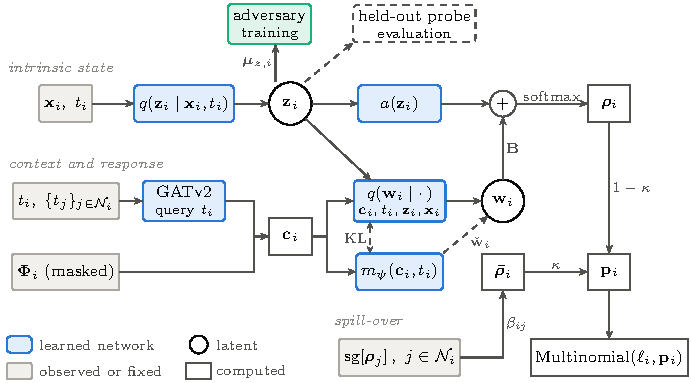
\includegraphics[width=0.65\textwidth]{recomb_fig_model_graph}
\caption{The computation graph of DISCELL for one cell $i$. $\vz_i$ is encoded from the cell's own counts and type; $\vc_i$ combines attention over the neighbours' types, queried with the cell's type, with $\vPhi_i$; $\vw_i$ has the prior $p(\vw_i \mid \vc_i, t_i)$ with mean $\mpsi$ and a posterior that also sees the cell. $\vrho_i$ is mixed with the neighbours' clean compositions, held under a stop-gradient (sg), through $\beta$ and the fixed $\kappa$. The dashed $\wbreve_i$ is the prior draw of the intrinsic path. The adversary acts on $\vmu_{z,i}$ during training; the held-out probe grades it afterwards.}
\label{fig:model-detail}
\end{figure}

\subsection{Design Choices}

\paragraph{The type as attention query.}
\label{app:mirror}
In the attention layer of \cref{eq:context-gat} the destination feature enters the attention weights but not the aggregated values \citep{brody2022}. Querying with $\vz_i$ would still open a selection channel: attention could weight neighbours by their similarity to $\vz_i$, so that $\vc_i$ mirrors the cell, $\mpsi$ already knows it, and the response divergence collapses, with $\vw_i$ measuring deviation from \emph{self}. The query is therefore the cell's type, at no cost to the prior, which receives $t_i$ anyway; the sources are the neighbours' types, chosen over types plus the neighbours' posterior means because a three-seed ablation favoured them. The \emph{mirror} diagnostic is the within-type $R^2$ of $\vz_i$ regressed on $\vc_i$ against a within-type permuted control; it must be ruled out before a vanishing response divergence is read as posterior collapse.

\paragraph{No per-edge geometry; Delaunay graph and Voronoi kernel.}
\label{app:graph}
The attention uses no distances or face lengths, so that it cannot rediscover the spill-over kernel $\beta$ and merge the two mechanisms. With the type as query and one-hot types as sources, the logit of edge $ij$ depends on $(t_i, t_j)$ alone, say $s_{t_i t_j}$, and per head
\begin{equation}
  \mathbf{g}_i = \frac{\sum_k y_{ik}\, e^{s_{t_i k}}\, \mathbf{W}_{\mathrm{src}}\mathbf{e}_k}{\sum_k y_{ik}\, e^{s_{t_i k}}},
  \label{eq:context-closed}
\end{equation}
a type-specific reweighting of the composition $\vy_i$ in which the degree cancels. The context thus depends on fractions, not counts; on a Delaunay graph the degree is nearly constant, so this costs little. Delaunay adjacency (Voronoi cells sharing a face) is built from centroids alone, with one parameter, the $40\um$ prune. A discretised contact indicator would not avoid the confound: on these sections, segmented mostly ($69$ to $87\%$ of cells) by an interior RNA stain, adjacent polygons rarely touch, and whether they do measures local density (\cref{tab:contact}). A contact kernel is zero on about half of the edges and leaves up to a third of the cells in the sparsest fifth of a section with no spill-over at all; the Voronoi-face kernel gives every connected cell the same budget $\kappa$. Edge features in the attention were not tested (\cref{app:limitations}).

\begin{table}[!htbp]
\centering
\caption{Segmented-polygon contact as a spill-over kernel against the Voronoi-face kernel $\beta$, on the model's edge set; both use the same distance decay and row normalisation. \emph{Touching}: adjacent polygons at zero distance; \emph{no contact}: edges with no membrane within $1\um$. \emph{No spill-over}: connected cells whose contact-kernel row is all zero; \emph{sparse}/\emph{dense}: lowest/highest fifth of cells by centroids within $20\um$. $\rho$: Spearman correlation over edges between a neighbour's share of the row and the gap between the polygons (decay alone: $-0.49$ to $-0.62$). The Voronoi kernel has no zero-weight edges on any section. FF: fresh frozen.}
\label{tab:contact}
\small
\setlength{\tabcolsep}{4pt}
\begin{tabular}{@{}lrrrrrrr@{}}
\toprule
& \multicolumn{2}{c}{Edges (\%)} & \multicolumn{3}{c}{No spill-over, contact (\%)} & \multicolumn{2}{c}{$\rho$(share, gap)} \\
\cmidrule(lr){2-3}\cmidrule(lr){4-6}\cmidrule(l){7-8}
Section & touching & no contact & all & sparse & dense & contact & $\beta$ \\
\midrule
Ovarian cancer (FFPE) & 3.5 & 47 & 9.8 & 33.6 & 0.6 & $-0.82$ & $-0.48$ \\
Lung cancer (FFPE) & 2.7 & 57 & 11.1 & 27.4 & 0.7 & $-0.84$ & $-0.55$ \\
Ovarian cancer (FF) & 6.7 & 38 & 3.2 & 10.6 & 0.1 & $-0.80$ & $-0.52$ \\
Lung TMA, section A & 2.2 & 47 & 6.3 & 24.8 & 0.1 & $-0.84$ & $-0.54$ \\
Lung TMA, section B & 2.2 & 47 & 6.2 & 24.6 & 0.1 & $-0.84$ & $-0.53$ \\
\bottomrule
\end{tabular}
\end{table}

\paragraph{The image descriptor and its mask.}
\label{app:image}
$\vPhi_i$ is the $384$-dimensional embedding by KRONOS \citep{kronos2025} (first release, ViT-S/16) of a $128\um$ field ($256$ pixels) in the section's four morphology channels. The channels map onto the model's marker vocabulary only approximately: the membrane and $\alpha$SMA channels are antibody mixes read as their named component, and 18S RNA is given an unused marker identity. The cell is removed by zeroing a disc of fixed radius centred on the crop anchor, not its own polygon, whose outline would reveal its type. A $25\um$ disc leaves six cells of the primary section outside it (elongated smooth-muscle cells, whose descriptor is set to zero) and masks $12\%$ of the field; at this density it also removes the first ring or two, so $\vPhi_i$ describes the tissue beyond roughly $25\um$. \Cref{tab:masking} shows what remains: the masked patch predicts the cell's label less well than the neighbours' labels alone, so what it knows about the cell is what its neighbourhood implies. On the masked patch the first release does at least as well as KRONOS2 at half the embedding width, so we use it.

\begin{table}[!htbp]
\centering
\caption{What each mask leaves in the image embedding (primary section): macro one-versus-rest AUC of a multinomial logistic regression predicting the cell's lineage label (11 classes) from the embedding, on a spatial split ($1\,$mm tiles, cells within half a field of a tile edge dropped; $40{,}000$ training and about $74{,}000$ test cells). The model uses KRONOS with the disc zeroed (bold).}
\label{tab:masking}
\small
\begin{tabular}{@{}lcc@{}}
\toprule
Input to the classifier & KRONOS & KRONOS2 \\
\midrule
Neighbours' labels, no image & \multicolumn{2}{c}{$0.918$} \\
Whole patch & $0.881$ & $0.878$ \\
Disc over the cell zeroed & $\mathbf{0.857}$ & $0.846$ \\
The cell alone & $0.905$ & $0.919$ \\
The cell alone, native resolution & $0.923$ & -- \\
\bottomrule
\end{tabular}
\end{table}

\paragraph{A direct path from the counts into $q(\vw)$.}
\label{app:qw}
The response posterior reads the cell's counts, because $\vw \perp \vx \mid \vz, \vc$ is false by explaining-away and $\vz$ is lossy in exactly the wrong direction: the invariance removes from it the niche-predictable variation that $\vw$ exists to capture. Without the path, $\vw_i$ collapses to the expected response given type and niche.

\paragraph{Conditional invariance and label granularity.}
\label{app:conditional}
The invariance of \cref{eq:invariance-target} is a constraint on the variational family, not a property of the generative model (\cref{app:posterior-reg}). It removes from $\vz$ only what the neighbour composition and the masked image predict given the type. Intrinsic variation that is spatially organised within a type, such as subclones in contiguous regions whose kin the masked image shows, is partly predictable from the niche, is moved into $\vw$ and would be read as a response; on a carcinoma section this is the main case, not a corner case. The decomposition is therefore relative to the labels. We use lineage-level labels because finer or state-defined labels leave $\vz$ little to carry and destroy the overlap that conditional comparisons need, and because $t_i$ is itself a function of the counts, so conditioning on it conditions on a descendant of the niche near label boundaries \citep{hernan2004}; marginal invariance instead collapses the agreement with type \citep{slavutsky2025}.

% S3: copied from ../aistats/appendix (see SETUP_REPORT.md for provenance); edit here, not there.
% Trimmed 2026-10-01 (agent A): continues the section opened in S2_design_rationale.tex (no \section here).
% Cut: tab:deviations, tab:deviations2, fig:batching, fig:probe and app:probe; \input{probe} moved to S4 (agent B).
% Calibration ledger added; facts from S1 (old S1.2, S1.4), this file and S8 (app:sensitivity).

\subsection{Architecture and Hyperparameters}
\label{app:architecture}

\Cref{tab:architecture} lists every network and every fixed quantity as implemented. All multilayer perceptrons use rectified-linear hidden units.



\subsection{Calibration}
\label{app:S-calibration}

Every weight was set once, on the primary section, and used unchanged on every section; \cref{app:sensitivity} refits the alternatives. \Cref{tab:S-calibration} records what was tuned, by which read, and where it was checked.

\begin{table}[!htbp]
\centering
\caption{Networks and fixed quantities. $G$ genes, $K$ types, $\dPhi$ image-embedding dimension.}
\label{tab:architecture}
\footnotesize
\begin{tabular}{@{}p{0.2\textwidth}p{0.27\textwidth}p{0.475\textwidth}@{}}
\toprule
Component & Input & Layers / value \\
\midrule
Count encoding & $\vx_i$ & $[\log(1 + \vx_i \tilde\ell/\ell_i),\ \log\ell_i]$, $\tilde\ell$ the median total \\
$q(\vz_i \mid \vx_i, t_i)$ & count encoding $\oplus \onehot(t_i)$ & $256 \to 256 \to 2\dz$, $\dz = 20$ \\
Type query $\embed(t_i)$ & $t_i$ & learned table, width $K$ \\
Attention sources & neighbour $j$ & $\onehot(t_j)$, width $K$ \\
Attention layer & sources, query & one bipartite GATv2 layer, $4$ heads $\times\, 32$, averaged, LeakyReLU slope $0.2$, no self-loops, no edge features \\
Context $\vc_i$ & & attention output ($32$) $\oplus\ \vPhi_i$ ($\dPhi = 384$) $\oplus$ isolation flag ($1$) \\
Prior mean $\mpsi(\vc_i, t_i)$ & $\vc_i \oplus \onehot(t_i)$ & $64 \to \dw$, $\dw = 6$ \\
$q(\vw_i \mid \cdot)$ & $\vc_i \oplus \onehot(t_i) \oplus \vz_i \oplus$ count encoding & $256 \to 2\dw$ \\
Decoder $a(\vz_i)$ & $\vz_i$ & $256 \to G$ \\
Loadings $\vB$ & $\vw_i$ & linear $\dw \to G$, no bias \\
Adversary heads & $\vmu_{z,i} \oplus \onehot(t_i)$ & two heads $64 \to 64 \to K$ (composition) and $\to \Ephi = K$ (image niche) \\
Image niche $\ephi_i$ & $12$ principal components of $\vPhi$ & soft $k$-means memberships $\softmax(-d^2/T)$, $T$ the median nearest squared distance; projection fitted on a $50{,}000$-cell subsample, $k$-means (four restarts) on all cells; frozen \\
Held-out probes & $\vmu_{z,i} \oplus \onehot(t_i)$ & ridge ($\lambda = 10^{-3}$) and perceptron $64 \to 64$ ($300$ Adam steps at $10^{-3}$, batches of $2{,}048$), per block against its own within-type permutation floor; fitted on at most $30{,}000$ training-tile cells \\
\midrule
Graph & & Delaunay adjacency; Voronoi faces measured within $30\um$ discs; prune at $40\um$ \\
Kernel $\beta$ & & $f_{ij}\exp(-d_{ij}/\tau)$, $\tau = 20\um$, row-normalised over in-edges \\
Prior scale $\sigma_w$ & & $1$ (fixed) \\
\midrule
Spill-over fraction $\kappa$ & & swept over $\{0, 0.05, 0.1, 0.2, 0.3, 0.4\}$; operating point $0.1$ \\
$\omega$ & & $1$ \\
$\alphaz$ & & $\tfrac12/\lbar$, $\lbar$ the section's median total \\
$\alphaw$ & & $0.1$, ramped linearly from $0$ over the first $30$ epochs \\
$\alphaa$ (adversary) & & $0.3$; six head updates per model update at learning rate $2 \times 10^{-3}$; composition weighted $\lambda_y = 3$ \\
\midrule
Tiles & & recursive median split into rectangles of $\leq 4{,}096$ cells ($2{,}048$ on the TMA core); $15\%$ of tiles held out \\
Optimiser & & Adam \citep{kingma2015adam}, learning rate $10^{-3}$, cosine annealing \citep{loshchilov2017}, gradient-norm clip $10$; $500$ epochs, patience $40$, for final fits and sweep alike \\
Evaluation & & every $5$ epochs on posterior means; checkpoint accepted if held-out reconstruction improves and $\vz$--type agreement $\geq 0.9\times$ its running maximum; none during the $\alphaw$ ramp \\
Hardware & & one NVIDIA GeForce RTX 4090 (24\,GB) per fit \\
\bottomrule
\end{tabular}
\end{table}

\begin{table}[!htbp]
\centering
\caption{What was calibrated, on which section, by which read. Primary: the ovarian FFPE section.}
\label{tab:S-calibration}
\footnotesize
\begin{tabular}{@{}p{0.13\textwidth}p{0.17\textwidth}p{0.35\textwidth}p{0.27\textwidth}@{}}
\toprule
Setting & Set on & Read & Checked \\
\midrule
$\alphaz = \tfrac12/\lbar$ & primary & ladder $\{\tfrac14, \tfrac12, 1, 2\}\times 1/\lbar$, read on the diagnostics of \cref{sec:selection}; $\tfrac12$ restores one charge of the $\vz$-divergence at $\omega = 1$ (\cref{app:pathb}) & -- \\
$\alphaw = 0.1$ & primary & at lower weights $\vw$ takes over type structure and the $\vz$--type agreement falls & $1/\lbar$ on primary and TMA core; $5/\lbar$, $10/\lbar$ on FF \\
$\alphaa = 0.3$, head steps & primary & nonlinear held-out probe, without loss in $\vz$--type agreement or held-out reconstruction; head strength judged by the probe, never by the heads' loss \citep{elazar2018} & doubled steps, width, ensemble \\
$\lambda_y = 3$ & primary & composition residual $4.6\%$ against $6.6\%$ at equal weights & $\lambda_y = 1, 5$ \\
% omega: devlog "Reproduction card" (round 2, omega in {0.5, 2} against 1, 40-epoch single-seed fits, closed-form penalty;
%   data/datasets/xenium_prime_ovarian_cancer_ffpe/experiments/calibration_round2.json, key "omega") and the AISTATS
%   appendix/calibration.tex ("Round 2"). Widths: d_z = 20 is "fixed throughout" in the same card, with no search on record;
%   d_w: devlog "d_w ablation" (2026-09-14) and "d_w = 8" (2026-09-15), runs/dw{2,3,8}_s{0,1,2} against the d_w = 6 sweep fits,
%   200-epoch budget, before the final configuration.
$\omega = 1$ & primary, development & $\{0.5, 1, 2\}$, one seed, short fits with the closed-form penalty: $0.5$ lowered the $\vz$--type agreement, $2$ raised reconstruction with more residual niche signal; at $1$ the two bounds weigh equally & $\omega = 0$ on all four sections \\
$\dz = 20$ & -- & fixed during development, not tuned & -- \\
$\dw = 6$ & primary, development & $\{2, 3, 6, 8\}$, three seeds each: likelihood and the $\vz$ reads unchanged over $\{2, 3, 6\}$; the response used one or two axes at every width; at $8$ more cycle signal in $\vw$ & not at the final configuration \\
\bottomrule
\end{tabular}
\end{table}




\paragraph{The invariance threshold is not met everywhere.} During development, a closed-form Gaussian estimate of the conditional mutual information, evaluated on the posterior means with $\vv_i = [\vy_i^{(-K)}, \mathrm{PC}_{12}(\vPhi_i)]$,
\begin{equation}
  \Pen = \textstyle\sum_t p(t)\cdot \tfrac{1}{2}\big[\logdet \Sighat_{\vv \mid t} + \logdet \Sighat_{\vz \mid t} - \logdet \Sighat_{[\vz,\vv] \mid t}\big],
  \label{eq:S-penalty}
\end{equation}
served in place of the adversary; it removes linear dependence only, and the nonlinear probe of a converged fit stayed above its floor, so the adversary replaced it. The development target for the adversary was a nonlinear residual of at most a quarter of that of the fit without the adversary, on both blocks and for both probe families. At the operating point the nonlinear probe exceeds that threshold on the composition block on three sections and on the image block on the TMA core; on the TMA core and the lung section the residual without the adversary is itself small, so a similar absolute residual is a larger fraction of it. The residual niche signal is therefore reported descriptively, in absolute terms and as a fraction of the fit without the adversary (\cref{tab:probe}), not as a pass or a fail.

\subsection{Training, Diagnostics and Seeds}

The adversary's image target $\ephi_i$ is a soft membership in $\Ephi = K$ image niches from $k$-means on the leading principal components of $\vPhi_i$, never on the raw embedding, where distances are noise-dominated; $\Ephi = K$ gives the two heads comparable difficulty. The composition head is weighted $\lambda_y = 3$, in the encoder term and in the heads' loss, because composition is the channel of the spill-over confound.

The response divergence is ramped because without the ramp the conditional prior can fail to open: the posterior of $\vw$ collapses within the first ten epochs onto a prior that ignores $\vc$, shown by a divergence at zero and no information between $\vw$ and the niche on held-out cells. Such dead-channel fits were discarded and re-seeded; none is among the final fits. The running maximum of the type agreement ratchets upward, so a checkpoint that buys reconstruction with type structure is rejected. Held-out cells are entire spatial tiles, because spatial autocorrelation passes the answer across a random split \citep{roberts2017}. Every fit is monitored by the mirror $R^2$ (\cref{app:mirror}), the response divergence per dimension, the held-out probe (\cref{eq:probe}), the $\vz$--type agreement, and two checks that $\vz$ has not collapsed onto the label: $\I(\vz;t)/H(t)$ is $0.82$ to $0.95$ on the final fits, the within-type share of the variance of $\vmu_z$ $0.60$ to $0.72$, and decoding from the cell's own $\vz$ rather than its type's mean gains $0.06$ to $0.17$ nats per count (\cref{tab:recon-modes}). The objective is not unimodal in the seed: repeated fits of one configuration can fall into different basins. Each seed also redraws the held-out split, the image principal components and the image-niche clustering. No seed is selected: figures use one seed fixed in advance, tables the mean with the range over seeds. A spill-over-subtracted encoder input, an attention sink and coupled weight decay are implemented but off in every reported fit.

\subsection{Tiles and the Two-Hop Halo}
\label{app:tiles}

Because $\rhobar_i$ needs $\vrho_j$, hence $\vw_j$, hence $\vc_j$, a training step for cell $i$ reaches two graph hops. The neighbours' responses are posterior draws from the same batched pass; dropping them would strip the local programme from $\rhobar_i$ and let $\vw_i$ absorb it, inflating apparent spatial effects. The neighbours' compositions enter under a stop-gradient, as in resolVI \citep{ergen2026resolvi}, which closes the feedback path through which $\vrho_j$ would be trained to absorb cell $i$'s residual. Batches are contiguous spatial tiles, whose halo is shared: a tile's cells are the seeds, on which the loss is evaluated; their neighbours (ring one) get context, response and clean composition; ring two contributes only types. Both rings are read from the kernel's own edge list, never from a distance query, so the halo and $\beta$ cannot disagree. One consequence: the ring of a training tile can contain cells of a held-out tile, whose counts then enter training as stop-gradient inputs with no loss. On our sections $0.8$ to $1.9\%$ of training seeds have a held-out neighbour, and $4.8$ to $10\%$ of held-out cells enter some training step in this way; within two hops, where only the type is used, the share of seeds is $1.8$ to $4\%$. We state the exposure rather than add a buffer, which would remove the same seeds.

% S4: copied from ../aistats/appendix (see SETUP_REPORT.md for provenance); edit here, not there.
\section{Data, Labels and Comparison Methods}
\label{app:experimental}
% from experimental.tex: Sections, Lineage Labels, Baselines, Assets and Licences, What the Model Needs

\subsection{Sections}
\label{app:sections}

\Cref{tab:sections} lists the sections of \cref{sec:setup}, and \cref{fig:sections} shows them. The lineage classes include Unassigned. On the ovarian FFPE section it also holds a low-depth class of mixed lineage that the curated annotation had named as a tumour subtype, which is why its share is the largest.

\begin{table}[t]
\centering
\caption{The sections. Median counts are per cell over the whole section. The TMA core and its serial section are one core of the microarray on two slides; no model is fitted to the serial section.}
\label{tab:sections}
\small
\setlength{\tabcolsep}{4pt}
\begin{tabular}{@{}llrrrrr@{}}
\toprule
Section & Role & Cells & Genes & Lineage classes & Unassigned (\%) & Median counts \\
\midrule
Ovarian cancer (FFPE) & primary & 407{,}120 & 5{,}101 & 12 & 10.3 & 178 \\
Lung cancer (FFPE) & fitted & 278{,}324 & 5{,}001 & 20 & 0.1 & 242 \\
Ovarian cancer (FF) & fitted & 1{,}157{,}637 & 5{,}001 & 10 & 4.3 & 1{,}401 \\
Lung TMA core & fitted & 69{,}422 & 5{,}001 & 30 & 4.2 & 279 \\
Lung TMA core, serial section & held out & 70{,}757 & 5{,}001 & 30 & 4.8 & 253 \\
\bottomrule
\end{tabular}
\end{table}

\begin{figure}[t]
\centering
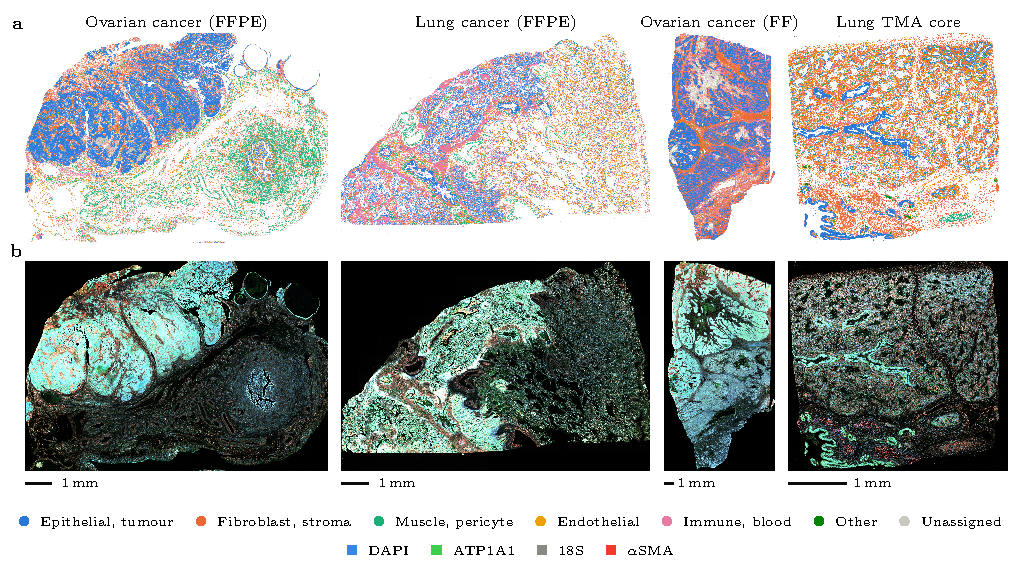
\includegraphics[width=\textwidth]{fig_sections}
\caption{The four fitted sections. \textbf{a},~Every cell at its centroid, coloured by its lineage label, with the labels grouped into six families for display only; the model is fitted with the finer lineage classes of \cref{tab:sections}. \textbf{b},~The morphology image of the same section, the four channels the image descriptor reads, shown as one colour composite (\cref{app:image}). The TMA panel is the fitted core only. Each section is shown at its own scale; the bars are $1$\,mm.}
\label{fig:sections}
\end{figure}

\subsection{Lineage Labels}
\label{app:lineage}

The fitted labels are lineage-level on every section (\cref{sec:setup}). States, such as proliferating, activated or hypoxic, and locations, such as tumour- or stroma-associated, are merged into their lineage; lineages and developmentally distinct sub-lineages are kept. The mappings were fixed and recorded before any model was refitted.

\paragraph{Curated annotations.}
On the ovarian FFPE section the eighteen curated classes become twelve (\cref{tab:lineage-ovarian}). Two classes needed a decision. The class named as a SOX2-OT$^+$ tumour subtype is mostly not tumour: its cells have a median of $27$ transcripts against $333$ for tumour cells, three quarters show no SOX2-OT count, and its pooled profile decomposes mostly into macrophage expression, so it is folded into Unassigned rather than into the tumour lineage. The class named as malignant cells lining a cyst expresses mesothelial markers (CALB2, PRG4, BNC1, PDPN, UPK3B) and lacks the tumour markers (EPCAM, PAX8, ESR1), and becomes its own lineage. On the lung TMA the thirty-five curated classes become thirty: the state classes (activated, inflammatory and myofibroblasts, activated endothelium and proliferating cells) are reassigned cell by cell to the sub-lineage their markers indicate, with the cell-cycle genes left out for the proliferating class, and the other classes are kept.

\paragraph{Other judgement calls.}
Four further choices are not forced by the rule and are stated so that they can be revisited. The tumour- and stroma-associated fibroblasts of the ovarian FFPE section are merged, because what separates them is the cancer-associated fibroblast programme, a state, rather than a lineage. Its two endothelial classes are merged too, although what separates them is less clear: a tip-cell state on one side and a weakly venous identity on the other. On the lung TMA the alveolar and adventitial fibroblasts are kept as distinct sub-lineages, and the myofibroblasts, which could belong to either, are split between them by their markers, about evenly. The cell-by-cell reassignment of the TMA's state classes is expected to be right for about three cells in four, and its margins are recorded with the mapping.

\paragraph{Clustered sections.}
On the lung FFPE section and the fresh-frozen ovarian section the labels start from unsupervised clusters, and each cluster is assigned the lineage its marker genes indicate, on the lung TMA's vocabulary for the lung section (\cref{tab:lineage-clusters}). Clusters of immune cells next to tumour that carry some tumour signal keep their immune lineage, since that signal is the spill-over the model is built to absorb, and one low-depth cluster of the fresh-frozen section becomes Unassigned.

\begin{table}[t]
\centering
\caption{Lineage labels on the ovarian FFPE section: the curated classes merged into each lineage.}
\label{tab:lineage-ovarian}
\small
\begin{tabular}{@{}>{\raggedright\arraybackslash}p{0.28\textwidth}>{\raggedright\arraybackslash}p{0.62\textwidth}@{}}
\toprule
Lineage & Curated classes \\
\midrule
Ciliated epithelial cells & Ciliated Epithelial Cells \\
Endothelial cells & Stromal Associated Endothelial Cells, Tumor Associated Endothelial Cells \\
Fallopian tube epithelium & Fallopian Tube Epithelium \\
Fibroblasts & Stromal Associated Fibroblasts, Tumor Associated Fibroblasts \\
Macrophages & Macrophages \\
Mesothelial-like cyst lining & Malignant Cells Lining Cyst \\
Pericytes & Pericytes \\
Smooth muscle cells & Smooth Muscle Cells \\
T/NK cells & T and NK Cells \\
Tumour & Inflammatory Tumor Cells, Proliferative Tumor Cells, Tumor Cells, VEGFA+ Tumor Cells \\
Unassigned & SOX2-OT+ Tumor Cells, Unassigned \\
Urothelial-like cells & Urothelial-like Cells \\
\bottomrule
\end{tabular}
\end{table}

\begin{table}[t]
\centering
\caption{Lineage labels on the two clustered sections: the clusters assigned to each lineage.}
\label{tab:lineage-clusters}
\small
\begin{tabular}{@{}>{\raggedright\arraybackslash}p{0.24\textwidth}>{\raggedright\arraybackslash}p{0.13\textwidth}@{\hspace{0.04\textwidth}}>{\raggedright\arraybackslash}p{0.2\textwidth}>{\raggedright\arraybackslash}p{0.33\textwidth}@{}}
\toprule
\multicolumn{2}{@{}l}{Lung cancer (FFPE)} & \multicolumn{2}{l@{}}{Ovarian cancer (FF)} \\
\cmidrule(r){1-2}\cmidrule(l){3-4}
Lineage & Clusters & Lineage & Clusters \\
\midrule
AT1 & 18, 23 & Endothelial cells & 16, 38 \\
AT2 & 20 & Fibroblasts & 7, 13 \\
Adventitial fibroblasts & 4, 17 & Macrophages & 10, 14, 19, 20, 25, 26, 28, 30, 34 \\
Alveolar fibroblasts & 10 & Ovarian stroma & 3, 6, 23 \\
Alveolar macrophages & 16 & Pericytes & 32 \\
B cells & 12 & Plasma cells & 17, 35 \\
EC general capillary & 3, 22, 25 & Smooth muscle cells & 33 \\
EC venous & 13 & T/NK cells & 18, 22, 24, 27, 29, 31, 36, 37 \\
Goblet & 19 & Tumour & 1, 2, 4, 5, 8, 11, 12, 15, 21 \\
Interstitial macrophages & 2 & Unassigned & 9; unclustered cells \\
Mast cells & 27 &  &  \\
Multiciliated & 26, 28 &  &  \\
Neuroendocrine & 31 &  &  \\
Neutrophils & 6 &  &  \\
Pericytes & 24 &  &  \\
Plasma cells & 15 &  &  \\
Smooth muscle & 5 &  &  \\
T/NK cells & 1, 7, 21, 30, 32 &  &  \\
Tumour & 8, 9, 11, 14, 29 &  &  \\
Unassigned & unclustered cells &  &  \\
\bottomrule
\end{tabular}
\end{table}

\subsection{Baselines}
\label{app:baselines}

\Cref{tab:baselines} gives the configuration of each comparison method. Every method is run at its published defaults, and on our pruned Delaunay graph where it accepts an external graph; resolVI and MintFlow build their own. The methods that read a label read the lineage labels. SIMVI does not read one, so refitting it at lineage labels only checks reproducibility. Every comparison is on whole sections: a method that cannot be fitted to a whole section on the resources available is reported as such, with the measured reason, and never on a window of the section. Cellina removes a spatial-domain label from its intrinsic latent adversarially, and our sections carry no such label, so its main row runs without the adversary. It is run in three further forms: with the adversary given our niche label (clusters of neighbour composition, $K = 10$, fitted on training cells), which matches what our probe grades and is therefore Cellina's best case on the probe, not its published setting; on its own neighbour graph instead of ours, on the TMA core and its serial section; and, for the counterfactual comparison of \cref{tab:cellina-cf}, refitted on the training tiles only and decoded at its posterior mean. \Cref{tab:battery} gives every method's values on one battery of reads. MintFlow's reconstruction is not reported: its stored value was found invalid, because an export error in our pipeline passed MintFlow's split of each cell's observed counts, which sums back to those counts, in place of a decode, so the read scored each cell against its own counts. MintFlow is being refitted on its three sections with a corrected export, and all its reads will be taken from the new fits \pending{MintFlow refits with the corrected export}. \Cref{tab:context} grades each method's context latent in the same way, in the positive direction: how much of the niche it carries.

\paragraph{Cellina variants.} Given our niche label as its domain, Cellina's adversary does not consistently lower its composition residual: the nonlinear residual falls on three sections of five and rises on the lung section and the TMA core, by at most $2.0$ points either way, the linear one rises on four sections of five, and its NMI with type and cycle $R^2$ fall on every section (\cref{tab:probe,tab:battery}). On its own neighbour graph, run on the TMA core and its serial section only, its composition residual is slightly higher than on ours and its cycle $R^2$ higher.

\begin{table}[t]
\centering
\caption{Comparison methods as run. Versions are the package versions used. \emph{Latents}: the latent each method's intrinsic read-outs are taken from, and the latent that plays the role of DISCELL's response $\vw$ in \cref{tab:context}. \emph{Coverage}: the sections with a completed whole-section fit, and the state of the others.}
\label{tab:baselines}
\small
\setlength{\tabcolsep}{4pt}
\begin{tabular}{@{}>{\raggedright\arraybackslash}p{0.1\textwidth}>{\raggedright\arraybackslash}p{0.15\textwidth}>{\raggedright\arraybackslash}p{0.12\textwidth}>{\raggedright\arraybackslash}p{0.1\textwidth}>{\raggedright\arraybackslash}p{0.15\textwidth}>{\raggedright\arraybackslash}p{0.26\textwidth}@{}}
\toprule
Method & Version & Graph & Label & Latents: intrinsic / context & Budget and coverage \\
\midrule
resolVI & scvi-tools 1.5.1 & own, 10 nearest neighbours & lineage & its single cell latent / none (neighbour spill-over is a mixture, not a latent) & 50 epochs; every section; on the serial section refitted there, since the transfer from the core failed \\
SIMVI & simvi 0.1.2 (scvi-tools 0.16.1) & ours & not used & intrinsic latent / spatial latent & package default; the TMA core, and the serial section fitted on itself. Could not be run on the resources currently available on the lung FFPE, ovarian FFPE and fresh-frozen sections: out of GPU memory on a 24 GB card within minutes (requests of $5.2$ GiB, $7.7$ GiB and $40$ MiB with $21.3$, $15.9$ and $23.5$ GiB in use) \\
MintFlow & mintflow 0.3.0 & own Delaunay graph & lineage & intrinsic latent / microenvironment latent & width 600, 50 epochs; the TMA core, transferred to its serial section, and the whole lung FFPE and ovarian FFPE sections; reconstruction not reported, refits with a corrected export running \pending{MintFlow refits with the corrected export}. Could not be run on the resources currently available on the fresh-frozen section ($1.16$ M cells): killed for lack of host memory after $574$ s of data set-up, before training, on a 125 GB host \\
Cellina & cellina 1.1.1 (scvi-tools 1.2.0) & ours & lineage & intrinsic latent / microenvironment latent $s$ & package default, no domain adversary; every section, transferred from the core to its serial section \\
Cellina, niche domain & as Cellina & ours & lineage; niche label as domain & as Cellina & as Cellina; every section \\
Cellina, own graph & as Cellina & own & lineage & as Cellina & as Cellina; the TMA core and its serial section \\
Cellina, counterfactual & as Cellina & ours & lineage & as Cellina & refitted on training tiles only; the four fitted sections \\
\bottomrule
\end{tabular}
\end{table}

\input{\tablesdir/battery}

\input{\tablesdir/context}

\subsection{Assets and Licences}
\label{app:assets}

The ovarian FFPE, lung FFPE and fresh-frozen ovarian sections are public datasets of 10x Genomics \citep{tenx_ovarian_ffpe,tenx_lung_ffpe,tenx_ovary_ff}, released under the Creative Commons Attribution 4.0 International licence (CC BY 4.0). The TMA core and its serial section are two public samples of GEO series GSE315411 \citep{williamskatek2026fishing}. The image model KRONOS and its successor KRONOS2 \citep{kronos2025} are released under CC BY-NC-ND~4.0, for non-commercial academic research and after registration; we use them as distributed by their authors, for that purpose, and redistribute neither. The comparison methods are released under the BSD 3-Clause licence: scvi-tools, which contains resolVI, SIMVI, MintFlow and Cellina. A code repository accompanies the submission as a clean, standalone implementation of DISCELL; it does not contain KRONOS or its weights, which are obtained from their authors under their licence. No new data are released.

\subsection{What the Model Needs}
\label{app:inputs}

Every fit in this paper is to a section profiled with Xenium Prime 5K. From its output the model uses five inputs (\cref{tab:inputs}). The graph needs positions only. It is the Delaunay adjacency of the cell positions, and the kernel's two ingredients, the length of the shared Voronoi face and the distance between positions, come from the positions too (\cref{app:graph}). The segmented polygons are therefore not required. Our runs take each cell's position as the centroid of its segmented polygon; the centroid the platform reports would serve equally in form. The polygons were used for three things outside the model: choosing the radius of the disc that removes the cell from the image field, which a new tissue or platform would need to recheck from its cell sizes (\cref{app:image}), and the graph and mask comparisons of \cref{app:graph,app:image}. The transcript coordinates, the nucleus boundaries and the H\&E image taken after the run are not used. Cell-cycle genes enter a diagnostic only (\cref{sec:selection}).

\begin{table}[t]
\centering
\caption{The inputs of a fit, and where they come from in a Xenium Prime 5K output.}
\label{tab:inputs}
\small
\begin{tabular}{@{}>{\raggedright\arraybackslash}p{0.22\textwidth}>{\raggedright\arraybackslash}p{0.38\textwidth}>{\raggedright\arraybackslash}p{0.34\textwidth}@{}}
\toprule
Input & Used for & Xenium Prime 5K source \\
\midrule
Counts per cell & the likelihood and the intrinsic encoder & the cell-by-gene count matrix \\
One position per cell & the graph, the kernel, the tiles and the image fields & the centroid of the segmented cell \\
Pixel size & every length in micrometres & the run's metadata \\
A type label per cell & the prior on the response, the adversary and the context's query & a curated annotation, or clusters of the counts mapped to lineages (\cref{app:lineage}) \\
Morphology image & the image descriptor $\vPhi_i$ & the four-channel morphology image \\
\bottomrule
\end{tabular}
\end{table}

\paragraph{Implicit requirements.} Counts must be assigned to segmented cells at single-cell resolution: the spill-over term models transcripts misassigned between neighbouring cells, and has no meaning for a unit that holds several cells. One fit is to one contiguous section. Counts are modelled as a multinomial given each cell's total, suited to the hundreds to about a thousand counts per cell of in situ data (\cref{sec:generative}), and a type label must be derivable for every cell. Nothing else is assumed about the gene panel.

\paragraph{Other assays (untested).} None of the following has been run. Each paragraph states what the model's assumptions would require, not what it would deliver.

\emph{Imaging platforms with other panels.} Other imaging-based assays, including smaller Xenium panels, provide segmented counts, positions and fluorescence stains, the inputs of \cref{tab:inputs}. The model applies in form. What changes is the depth and number of genes, and the stains, whose mapping onto the image model's marker vocabulary would have to be redone (\cref{app:image}).

\emph{Sequencing-based arrays.} On a high-resolution array whose bins are assigned to segmented cells, counts per cell and positions are available, but two things differ. The image is H\&E rather than multiplexed fluorescence, so the image descriptor would need an H\&E encoder. And transcripts are also mislocated by lateral movement during capture, a mechanism separate from segmentation whose extent differs between platforms: small on one high-resolution array \citep{deoliveira2025visiumhd}, larger on another \citep{ren2025benchmark}. The form of the spill-over kernel would have to be re-examined before the sweep could be read the same way. Arrays whose spots hold several cells pose a deconvolution problem rather than a spill-over problem and are outside the model's setting.

\emph{Protein imaging.} Multiplexed protein imaging measures intensities per marker rather than counts, so the multinomial likelihood would have to be replaced. The spill-over mechanism carries over, since signal from a neighbour's membrane spills over into the cell, through imperfect segmentation and through the interleaving of adjacent membranes \citep{bai2021redsea}, and the image model was built for such images \citep{kronos2025}, so the image descriptor would be native to the assay.

% S5: copied from ../aistats/appendix (see SETUP_REPORT.md for provenance); edit here, not there.
% Trimmed 2026-10-01 (agent B): see _reports/trim_B.md.
\section{Readout Definitions}
\label{app:readouts-section}
\subsection{Readouts}
\label{app:readouts}

Every readout is taken at the accepted checkpoint of each fit. Unassigned cells are never targets but remain neighbours. A readout is the mean over three seeds with the range; unless stated otherwise its interval is from a bootstrap over $200\um$ squares (tiles) of the section ($1{,}000$ draws, conditional on the fitted model and probes), reported as the envelope of the seeds' intervals (\cref{tab:headline-full}).
\input{\tablesdir/headline_full}

\paragraph{Niches.} Where a readout needs discrete niches, they are the ten clusters of a $k$-means clustering of the neighbour composition $\vy_i$ of connected cells; isolated cells have none.

\paragraph{Diagnostics.} The \emph{mirror $R^2$} is the pooled $R^2$ of a linear regression of $\vmu_z$ on the context $\vc_i$, both centred per type, on up to $30{,}000$ cells (\cref{sec:selection}). The response's information about the niche, $\I(\text{niche}; \vw)$, is a nearest-neighbour estimate \citep{ross2014} of the mutual information between the niche label and $\vmu_w$ on up to $20{,}000$ held-out cells, in nats, minus its mean over five permutations of the label within type. The \emph{cycle scores} are the S and G2/M scores of the gene sets of \citet{tirosh2016} intersected with the panel: each the mean depth-normalised log expression of the set minus that of expression-matched control genes, from the cell's own segmented counts \citep{wolf2018}. They are a proxy for the cycle, not a measurement of it: the counts also hold transcripts spilled over from neighbours and expression induced by the environment, and both enter the scores (\cref{sec:results-z}). The cycling set is the tenth of held-out cells with the highest summed score, fixed per section for every method, plus the training cells scoring above its lowest member. The \emph{cycle $R^2$} of a latent ($\vmu_z$, or $\vmu_w$ for the cycle asymmetry of \cref{app:sweep}) is that of a ridge regression of both scores, centred per type within the set, on the latent, fitted on the set's training cells and scored on its held-out cells; the linear reference regresses on the leading $50$ principal components of the log-normalised counts.

\paragraph{Relocation.} A panel is a cell type and a pair of niches $A$ and $B$, each with at least $500$ cells supplying model quantities and $100$ cells of the type to score; tiles are dealt into five spatial folds, one scored and four supplying every model quantity. Per gene, the observed shift is the difference between the two niches in the logarithm of the type's mean depth-normalised counts. The prediction holds niche $A$'s intrinsic rate fixed and adds two channels: the \emph{programme part}, $\vB$ times the difference between the mean prior means $\mpsi(\vc_i, t)$ of the type's cells in $B$ and in $A$, and the \emph{spill-over part}, the change in the logarithm of the mixture of \cref{eq:gen-p} when $A$'s mean spill-over influx is replaced by $B$'s at the fit's $\kappa$. No cell's own posterior response enters. A panel's \emph{score} is the $R^2$ of the prediction against the observed shift, both centred over the genes expressed in both niches; the same score is computed for each part alone. The \emph{noise ceiling} is the Spearman--Brown reliability of the observed shift from two random halves of the scored cells, averaged over four splits. Panels enter when their niches differ by more than three standard deviations of composition along the line between them; a panel is \emph{trusted} when its ceiling is at least $0.5$ with at least $100$ genes scored. The \emph{fraction of the ceiling} is the mean score over the trusted panels divided by their mean ceiling; over all panels the ratio divides by near-zero ceilings and can exceed one, so it is reported only in \cref{tab:transport-heldout}. The parts of \cref{tab:cellina-cf} are the same ratio for each part alone; they are separate scores and do not add up. The breakdown contrast of \cref{app:sweep} uses the mean score over all panels, without the trust filter: that of the full prediction minus that of the spill-over part alone (and, as a trajectory, minus that of the programme part alone, which is zero at $\kappa = 0$ by construction).
% source: scripts/logs/breakdown_2026-09-29/FAMILY.md, members transport_cf_minus_leak (ALL panels, mean R2(program + leak_only) - mean R2(leak_only)) and transport_cf_minus_program (trajectory only).
The interval recomputes shifts, scores and ceilings on half of the tiles drawn without replacement and rescales the spread to the full section. On planted sections with tile-clustered noise its coverage is $0.94$ to $0.96$ at ceilings of $0.82$ and $0.85$, but $0.78$ to $0.88$ at ceilings of $0.52$ to $0.63$, just above the trusted threshold, so at the ceilings of real panels it is closer to an $80\%$ than a $95\%$ interval.
% source (audit item 15): planted-coverage table (400 simulated sections x 200 draws), scripts/logs/final_repair_2026-09-27/AGENT_REPORT.md section 5; simulated sections have no Unassigned class, so the table does not depend on the mask; the interval method is unchanged since.
Splitting the reliability halves by tiles instead of cells raises the trusted fraction by $0.01$ to $0.02$ on the seed mean of the ovarian FFPE, lung and fresh-frozen sections ($-0.03$ to $+0.05$ in single fits) and leaves the TMA core with no trusted panel; with the cell split, the TMA core has a trusted panel on two of its three seeds.
% source (audit item 15): runs/finalL_s0-s2/transport/transport.json, summary.extrapolation_trusted.counterfactual_of_ceiling against summary.extrapolation_trusted_tiles.fraction_of_ceiling_tiles, post-mask reads (eval_mask Unassigned, written 2026-09-28 16:17 to 2026-09-29 03:55); the devlog's pre-mask "+0.01 to +0.03" (2026-09-28) is not used.

\paragraph{Single-cell read and twin read.} On the same panels, without the trust filter, up to $2{,}000$ held-out cells of the type in $A$ are decoded from their own $\vmu_z$ at $B$'s mean prior response and influx (the moved cloud) and at $A$'s (the cloud left in place); the type's held-out cells in $B$, decoded at their own posterior means, context and influx, are the target. The \emph{single-cell read} is the gap closed, $(U - T)/(U - F)$, where $T$ and $U$ are the maximum mean discrepancies \citep{gretton2012} of the moved cloud and of the cloud left in place from the target, under a Gaussian kernel on square-root profiles, and $F$ that between two random halves of the target; it is clipped to $[-1, 1]$ and summarised by its median over panels. Its \emph{type-mean reference} is the same gap closed with the moved cloud replaced by copies of the target's mean profile; the breakdown contrast is the single-cell read minus this reference. Its interval resamples the tiles of the source cells. The \emph{twin read} matches each target cell to the moved source cell nearest to it in $\vmu_z$; with $d_{\mathrm{twin}}$ and $d_{\mathrm{rand}}$ the median Hellinger distances from the target cells' own decodes to their matches and to random moved source cells, a panel's margin is $(d_{\mathrm{rand}} - d_{\mathrm{twin}})/d_{\mathrm{rand}}$, summarised by its median over panels; its interval resamples the tiles of the target cells. Because the decode is continuous in $\vz$, part of this margin follows from the construction.
% source: discell/model/transport.py twin read (margin = (median random - median transported)/median random per panel; summary median over panels); FAMILY.md readB_twin_margin.

\paragraph{Response programmes.} The programmes are the principal directions of the within-type-centred response that carry at least $1\%$ of its variance, rotated by varimax \citep{kaiser1958} in gene space; their number is the effective rank. The cross-seed cosine compares the first programme's gene signature between seeds; the programme overlap compares the gene subspaces two fits' programmes span. Localisation compares each programme's absolute loadings on four Gene Ontology cellular-component sets \citep{ashburner2000,go2023} with the rest of the panel (Mann--Whitney, Benjamini--Hochberg within a fit \citep{benjamini1995}; effect: rank-biserial correlation).

\paragraph{External criteria.} \emph{Signalling-gene share}, after MintFlow \citep{akbarnejad2025mintflow}: on the relocation panels each gene's observed shift is split into response part, spill-over part and remainder, and each gene's share of each part is accumulated over panels; ligand and receptor genes of a curated database \citep{jin2025cellchat} are compared with the other genes by a Mann--Whitney test, and the breakdown contrast is the rank-biserial effect for the response share (interval by half-tile subsampling). \emph{Niche information of both latents}: $\I(\text{niche}; \cdot)$ as above for $\vmu_z$ and $\vmu_w$, also by a neural estimator \citep{belghazi2018}. \emph{True and false axis}, after SIMVI \citep{dong2025simvi}, on the sections with tumour cells (the TMA sections have none): cells are banded by the fraction of tumour cells among their $50$ nearest neighbours, in six bands. For each gene and type, the response-predicted shift per band, from the prior means of the type's cells, is correlated by Kendall's $\tau$ with the band index (the true axis) and with equal-count bins of the in-plane coordinate least correlated with the band index (the false axis); the breakdown contrast is the mean $|\tau|$ over all gene--type pairs on the true axis minus that on the false axis. The same is done for shifts predicted from the intrinsic state and from depth, and for the observed shift. The false axis is not orthogonal to the bands: both in-plane coordinates correlate with the band index at about $0.41$.
% source: FAMILY.md (axis test on ovarian FFPE, lung FFPE and ovarian FF from 2026-10-01; not applicable on both TMA sections, no tumour lineage); discell/experiments/external_criteria.py pooled mean_abs_tau_true / _false over concatenated gene-type pairs.

\paragraph{Marker pairs.} After resolVI \citep{ergen2025}: twelve marker pairs that should not be co-expressed and six or seven control pairs that are, fixed per section before the read, are scored on held-out cells. A pair is double positive in the raw counts when both genes have a count, and in the corrected decode when both of $(1-\kappa)\,\ell_i\rho_{ig}$ round to at least one. The marker-pair contrast, a trajectory (\cref{app:sweep}), is the change in the exclusive pairs' double-positive rate from the raw counts to the corrected decode, minus the same change for the control pairs.

\subsection{Programme Scores and Drivers}
\label{app:S-drivers}

A cell's \emph{score} on programme $k$ is its coordinate along that programme of the within-type-centred $\vmu_w$, scaled to unit variance and signed so that the programme's largest loading is positive; the leading programme of a section is the one with the largest share of the response's within-type variance in the first seed's fit. Its \emph{Moran's I} is $\mathbf{u}^\top \mathbf{W}\mathbf{u} / \mathbf{u}^\top\mathbf{u}$ for the scores $\mathbf{u}$, centred per type, under the row-normalised adjacency $\mathbf{W}$ of the model's graph restricted to target cells; the Moran's I of a latent is defined in \cref{app:moran}.
% source: discell/model/atlas.py:centred_program_basis (whitened u, order by variance share, sign); build_atlas (morans_i on center_per_type(u) over connected targets, row_normalised_graph); validate.py:morans_i. Leading = programs[0] of finalL_s0: aistats/figures/src/recomb_fig_programmes.py:leading_summary.

The drivers regress the score on three blocks of the cell's context, each centred per type: the neighbour composition $\vy_i$ on the graph; the first $12$ principal components of the image embedding $\vPhi_i$; and $\ln(1 + \min(d, 500\um))$, with $d$ the distance to the nearest cell of each landmark class. The classes, built from the type labels and positions only, are: vessels, every cell type named endothelial (with the pericytes when at least half of them lie within $30\um$ of an endothelial cell); smooth muscle, each smooth-muscle type kept only in compact groups of $20$ to $500$ cells (density clustering at $40\um$); and the tumour--stroma interface, the cells on graph edges that cross the boundary where the share of tumour cells among the $50$ nearest cells passes one half. A vessel or smooth-muscle class with fewer than five groups of at least $20$ cells is dropped, as is the interface on sections without tumour cells; a section without any class has no landmark block. In the final fits both ovarian sections have all three classes, the lung FFPE section smooth muscle and the interface, and the TMA core vascular smooth muscle only; the endothelium of the two lung tissues carries a label the vessel rule does not match, so they have no vessel class.
% source: atlas.py:landmark_distance_block (log1p(min(d, 500)), cKDTree nearest constituent) and build_atlas (y = data.graph.y, PCA(12) of phi fitted on 50k cells; blocks center_per_type over all cells); validate.py:landmark_inventory (DBSCAN eps 40 um, min_samples 8, instances >= 20, smooth muscle <= 500, >= 5 instances; interface kNN k = 50, > 0.5) and _dbscan_instances; labels.py:is_endothelial / is_smooth_muscle / is_tumour (name regexes).
% classes kept on finalL_s0: ovarian FFPE and FF vessels + smooth muscle + interface; lung FFPE smooth muscle + interface; TMA core vascular smooth muscle only (atlas.json landmark_classes).
% CAVEAT (open): the lung FFPE and TMA sections do have endothelium, labelled "EC ..."; the endothelial name matcher misses it, so their vessel class is absent by a matching gap, not by annotation.

On up to $30{,}000$ connected target cells, each block alone, all three together, and all but one are fitted by ridge regression on standardised features ($\lambda = 10^{-3}$) over five folds of whole tiles, each tile assigned to one fold in turn. $R^2$ is one minus the variance of the held-out residual over that of the score; a block's \emph{unique} $R^2$ is the joint $R^2$ minus that without the block (drawn at zero when negative).
% source: atlas.py:context_drivers (marginal, joint, partial = joint - rest) and build_atlas (sample = connected & targets, <= 30,000); validate.py:ridge_cv (lam 1e-3, fold-train z-scoring, intercept), r2, collect_latents (fold = tile index mod 5 over training and validation tiles). Clipping at 0: recomb_fig_programmes.py panel c.

\subsection{Merged Subtypes}
\label{app:subtype}

Within each lineage that absorbed at least two curated classes or clusters, those become sublabels (each with at least $20$ training and $10$ held-out cells). Probes fitted on training tiles predict the sublabel on held-out tiles from $\vmu_z$, $\vmu_w$, the prior mean $\mpsi(\vc_i, t_i)$ and both latents: a class-balanced ridge classifier (primary) and, per latent, a small perceptron. Two scores are read: per lineage the \emph{balanced accuracy} (the main text's figure; chance $1/K$ for $K$ sublabels), and per sublabel the one-versus-rest \emph{AUC} against the rest of its lineage, with a floor from five within-lineage permutations of the sublabels and a tile-bootstrap interval, on which the call is made. The call, fixed before the first read: a channel recovers a sublabel when the lower end of its interval is above its floor; channel $a$ is far ahead of $b$ when the interval of their difference is above zero and $b$'s excess over its floor is at most half of $a$'s; the call is the majority over seeds. Only the curated sublabels of the primary section and of the TMA core carry an expected allegiance (a state to $\vz$, a location to the response); the clusters of the lung and fresh-frozen sections are read for information. The primary section's cyst lining is its own lineage, so every channel reads it through the type and its allegiance cannot be tested.

\begin{table}[!htbp]
\centering
\caption{Merged subtypes on the primary section: balanced accuracy of the held-out ridge classifier of the sublabel within each lineage, by channel. Mean over three seeds, range in brackets. $K$: number of sublabels; chance is $1/K$. The tumour lineage holds three curated states and the unqualified tumour class.}
\label{tab:S-subtype-ba}
% source: data/datasets/xenium_prime_ovarian_cancer_ffpe/experiments/subtype_recovery.md (written 2026-09-28 23:27, runs finalL_s0-s2), table "Balanced accuracy per lineage", ridge columns.
\small
\setlength{\tabcolsep}{4pt}
\begin{tabular}{@{}lccccc@{}}
\toprule
Lineage ($K$) & $\vmu_z$ & $\vmu_w$ & $\mpsi(\vc_i, t_i)$ & $\vmu_z \oplus \vmu_w$ & Chance \\
\midrule
Fibroblasts (2) & 0.66 [0.62, 0.68] & 0.95 [0.93, 0.97] & 0.94 [0.93, 0.96] & 0.95 [0.94, 0.97] & 0.50 \\
Endothelial cells (2) & 0.67 [0.65, 0.68] & 0.90 [0.88, 0.91] & 0.89 [0.88, 0.90] & 0.90 [0.88, 0.92] & 0.50 \\
Tumour (4) & 0.79 [0.78, 0.80] & 0.41 [0.40, 0.44] & 0.39 [0.32, 0.45] & 0.81 [0.80, 0.83] & 0.25 \\
\bottomrule
\end{tabular}
\end{table}

On the primary section (\cref{tab:S-subtype-ba}) the response separates the tumour- from the stroma-associated fibroblasts and endothelial cells, and its prior mean does so nearly as well; $\vz$ reads the tumour states. A perceptron on $\vmu_z$ reads more of the locations ($0.71$ and $0.78$) and of the states ($0.85$) without changing the dissociation. By AUC, the locations are read from the response at $0.96$ to $0.99$ against $0.71$ to $0.72$ from $\vz$, called on two seeds of three, and the proliferating and inflammatory states from $\vz$ at $0.96$ to $0.97$ against $0.61$ from the response, on every seed. The exceptions are states that also occupy a region: VEGFA$^+$ tumour cells are read from $\vz$ ($0.96$) and also from the response ($0.82$), and on the TMA core the myofibroblasts among adventitial fibroblasts are read better from the response than from $\vz$ ($0.92$ against $0.77$). On the fresh-frozen section three tumour-state clusters are read from both ($0.90$ to $0.96$ from $\vz$, $0.77$ to $0.86$ from the response).
% source: subtype_recovery.md as above ("Per sublabel: one-vs-rest AUC" and MLP mu_z balanced accuracy 0.71 / 0.78 / 0.85); other sections' AUCs unchanged from the previous text of this subsection.
The response and its prior mean give nearly the same AUC for every sublabel on the ovarian FFPE, fresh-frozen and TMA sections (within $0.07$, $0.01$ and $0.06$), the per-cell channel being closed (\cref{sec:results-w}); the one TMA exception is activated against venous endothelium, which the prior mean separates better ($0.76$ against $0.59$, on the one gradable seed). On the lung section the response separates clusters within three lineages better than its prior mean (AT1, $0.67$ against $0.55$; multiciliated cells, $0.71$ against $0.57$; one tumour cluster, $0.73$ against $0.59$), although its own deviation adds no more to reconstruction there than elsewhere (\cref{tab:recon-modes}) and $\vz$ separates all three better still ($0.90$): there the response readouts are not only readouts of the context regression.

% S7: copied from ../aistats/appendix (see SETUP_REPORT.md for provenance); edit here, not there.
\section{Simulation and Planted Tests}
\label{app:simulation}
% from synthetic.tex (whole) and experimental.tex: Planted Worlds
\subsection{Synthetic Recovery}
\label{app:synthetic}

\paragraph{Goal.} Check, on data simulated from the model's own generative story, that the final configuration recovers the planted intrinsic states, responses and gene programmes, that the adversary keeps the planted niche out of $\vz$, and how much a wrong spill-over fraction costs. A second simulation (\cref{app:planted-percell}) asks whether the response channel detects a per-cell response that the niche does not predict.

\paragraph{Generative process.} $N = 6{,}000$ cells uniformly in a $1{,}000\um$ box; $K = 8$ types assigned by a soft Voronoi partition around random anchors with Gumbel noise so that types cluster in space; the graph, kernel, composition and rings built by the same procedure as for real data from a Delaunay triangulation, with unit face lengths so that $\beta \propto \exp(-d/\tau)$ only; $\vz_i \sim \N(\mathbf{m}_{t_i}, 0.5^2\vI)$ with type means $\mathbf{m}_t \sim \N(\mathbf{0}, 1.5^2\vI)$; a planted response $\vw_i = \mathbf{M}^\top\vy_i + 0.3\,\boldsymbol\varepsilon_i$ linear in the true neighbour composition; $\log\vrho_i = \mathbf{A}\vz_i + \vB\vw_i$ (up to normalisation) with standard-normal loadings; $\rhobar_i$ the kernel-weighted neighbour average; $\vp_i$ the renormalised mixture at the planted $\kappa$; totals $\ell_i \sim \max(\Pois(150), 20)$; $\vx_i \sim \Mult(\ell_i, \vp_i)$; and a planted image descriptor $\vPhi_i = \mathbf{P}^\top\vy_i + 0.4\,\boldsymbol\varepsilon'_i$ in eight dimensions. $G = 60$ genes, planted $\dz = 4$, $\dw = 2$. Three worlds, drawn from three simulator seeds, at each planted $\kappa \in \{0, 0.2\}$.

\paragraph{Fit.} The final configuration (\cref{tab:architecture}), with the widths reduced to the small world ($\dz = 8$, $\dw = 2$, hidden width $128$, attention width $16$) and tiles of $512$ cells: the adversary at $\alphaa = 0.3$ with its composition term weighted three times, $\alphaw = 0.1$ with its warm-up over thirty epochs, $\alphaz = \tfrac12/\lbar$ with $\lbar$ the simulated section's median count ($150$, so $\alphaz \approx 0.0033$), $\omega = 1$, and the budget of $500$ epochs with patience $40$, with $15\%$ of the tiles held out for the stopping rule of \cref{sec:selection}. Every readout is taken on all cells at the accepted checkpoint. The uncontrolled arm is the same fit at $\alphaa = 0$. Each world is fitted with three model seeds, so every arm has nine fits. In the misspecified arms, the worlds planted at $\kappa = 0.2$ are fitted at each assumed $\kappa \in \{0, 0.1, 0.2, 0.3, 0.4\}$.

\paragraph{Readouts.} The agreement with the planted type, as the normalised mutual information between the planted types and a $k$-means clustering of $\vmu_z$ with $k = K$, against two references: the same clustering of the leading principal components of the log-normalised counts, which is what the counts alone support, and of the planted $\vz$ itself; the first canonical correlation between $\vmu_w$ and the planted response; the largest principal-angle cosine between the column spaces of the fitted and the planted loadings, against random two-dimensional subspaces of $\R^{60}$, whose cosine has a mean of $0.23$ and a $95$th percentile of $0.37$ to $0.38$ over $2{,}000$ draws; and the within-type coefficient of determination of the centred neighbour composition on $\vmu_z$, which is zero for the planted $\vz$.

\paragraph{Result.} At the matched spill-over fraction the final configuration recovers each planted quantity on every world (\cref{tab:synthetic}). The agreement of $\vmu_z$ with the planted type is $0.80$ to $0.96$, about what the counts support or more ($0.69$ to $0.93$; above the world's count clusters in seventeen fits of eighteen, and below them in one, $0.80$ against $0.83$) and short of the planted $\vz$ ($0.91$ to $0.98$), which is not reachable at $150$ counts per cell. The response correlates with the planted one at $0.83$ to $0.95$. The loadings are recovered above the random reference in every fit, at a cosine of $0.63$ to $0.99$; their recovery varies between seeds on some worlds, at both planted spill-over fractions (one fit of one world at $\kappa = 0$ reaches only $0.63$), which is why no gene-level statement on tissue is made from one fit (\cref{sec:sweep}). The intrinsic state carries almost none of the planted niche: the within-type $R^2$ of composition on $\vmu_z$ is at most $0.04$, against $0.11$ to $0.19$ without the adversary. Without the adversary the response and the loadings are also recovered worse and less reliably (canonical correlation $0.29$ to $0.91$, loadings $0.14$ to $0.85$). An earlier development run, at a configuration that is no longer used, had suggested that the loadings are bistable between seeds under a planted spill-over and stable without one; at the final configuration the spread between seeds is wider without a planted spill-over than under one: per world, the cosines span $0.63$ to $0.99$, $0.97$ to $0.99$ and $0.70$ to $0.98$ at $\kappa = 0$, against $0.98$ to $0.99$, $0.99$ and $0.77$ to $0.99$ at the matched $\kappa = 0.2$. Fitted at a wrong spill-over fraction, anywhere from $0$ to $0.4$ on worlds planted at $0.2$, the recovery moves little (\cref{fig:synthetic-misspec}): agreement $0.79$ to $0.97$, canonical correlation $0.78$ to $0.94$ (the lowest at an assumed $\kappa = 0$), loadings $0.71$ to $1.00$, composition $R^2$ at most $0.01$. On these worlds a spill-over fraction wrong by up to $0.2$ in either direction costs little of what is recovered. This also means that recovery does not point to the planted spill-over fraction, and it says nothing about spill-over of a form the model cannot represent.

\paragraph{Simulator checks.} Spill-over raises the kernel-weighted cosine between a cell's composition and its neighbours' by $0.22$ to $0.26$ at $\kappa = 0.4$ relative to $\kappa = 0$; the planted response is linearly predictable from composition ($R^2$ of $0.75$ to $0.87$); and the mixture is exactly the renormalised convex combination. These worlds have no isolated cells, so the reduction of the mixture to $\vrho$ for an isolated cell is not exercised here.

\input{\tablesdir/synthetic}

\begin{figure*}[t]
\centering
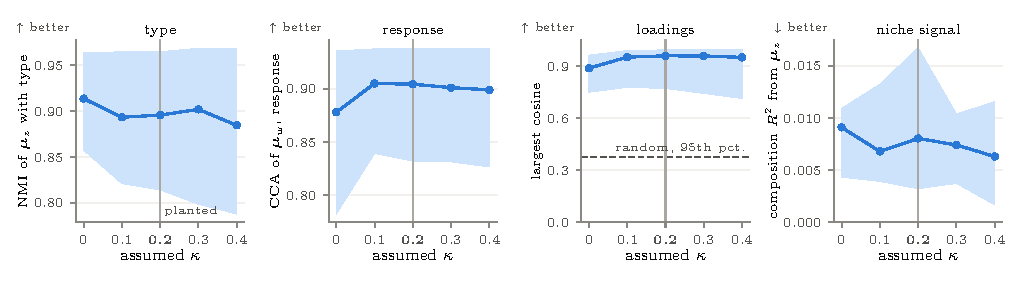
\includegraphics[width=\textwidth]{recomb_fig_synthetic_misspec}
\caption{Recovery on the worlds simulated at $\kappa = 0.2$, fitted at each assumed $\kappa$: NMI of $\vmu_z$ with the planted type; the first canonical correlation of $\vmu_w$ with the planted response; the largest principal-angle cosine of the fitted against the planted loadings (dashed: the $95$th percentile of random subspaces); the within-type $R^2$ of neighbour composition on $\vmu_z$. Line: mean over nine fits, three worlds with three model seeds each; band: their range, which is mostly the spread between worlds. The vertical line marks the planted value. Arrows point toward the better direction. The values are in \cref{tab:synthetic}.}
\label{fig:synthetic-misspec}
\end{figure*}

\subsection{A Planted Per-Cell Response}
\label{app:planted-percell}

At the operating point the response posterior adds almost nothing on the four sections: about one part in a thousand of held-out reconstruction (\cref{tab:recon-modes}), and a per-cell divergence whose ranking of cells does not reproduce between seeds (\cref{app:kl-maps}). Either these tissues carry little per-cell response beyond what the niche predicts, or the weight $\alphaw = 0.1$ closes the channel whatever the data (\cref{app:pathb}). On tissue the two cannot be told apart, so we plant a per-cell response and ask whether the channel finds it.

\paragraph{The plant.} On the worlds planted at $\kappa = 0.2$ above, in $10\%$ of the cells of the most abundant type, drawn at random and therefore spread across niches, the log-rate is shifted along the first axis of the planted response programme, with norm $s$ times the size of the planted niche effect (the root mean square over cells of the planted niche shift of the log-rate), for $s \in \{0, 0.5, 1, 2\}$; $s = 0$ is the recovery world itself. The subset cannot be predicted from neighbour composition, nor from composition and the image descriptor: a five-fold cross-validated classifier within the planted type reaches an AUC of $0.44$ to $0.54$ on all three worlds. The shift lies inside the planted response programme deliberately. A per-cell shift unrelated to the niche is something the intrinsic state may legitimately carry, since the invariance only keeps the niche out of $\vz$; a shift along the response programme is a cell responding more or less strongly than its niche predicts, which is what the per-cell channel exists to carry. The fit is the final configuration unchanged, with three model seeds on world 0, and, as a replication outside the rule, on worlds 1 and 2.

\paragraph{The rule, fixed in advance.} The channel detects a response of strength $s$ if, on world 0, every seed separates the planted cells from the other cells of their type by their response divergence $\KL(q(\vw_i)\,\|\,p(\vw_i \mid \vc_i, t_i))$ with an AUC of at least $0.8$, and every pair of seeds ranks the cells' divergences with a Spearman correlation of at least $0.5$. The smallest $s$ detected was to be reported; if none were detected, that finding would be reported instead: at this weight the channel is closed by design, not by the data.

\paragraph{Result.} No strength is detected, on world 0 or on either replication (\cref{fig:planted-percell}, \cref{tab:planted-percell}). The divergence separates the planted cells only partly and not on every seed (AUC $0.66$ to $0.85$ at $s = 1$ and $0.56$ to $0.69$ at $s = 2$ on world 0), and a plant does not make the seeds agree more on the per-cell divergences: on world 0 they agree less at $s = 0.5$ and $s = 1$ than without a plant (Spearman $0.34$ to $0.36$ and $0.11$ to $0.18$, against $0.39$ to $0.41$ at $s = 0$) and about as much at $s = 2$ ($0.25$ to $0.42$); on world 1 they agree less at every strength, and on world 2 about as much as without a plant. The rule's agreement criterion is read over the whole map, and even the null does not reach it. The response's own deviation from its prior mean moves toward the plant, but weakly (correlation $0.11$ to $0.41$ for $s > 0$ over the three worlds), and the held-out gain from it on the planted cells stays below $0.02$ nats per count. As the plant grows, it is increasingly absorbed by the intrinsic state instead: read through the decoder along the planted direction, the correlation of $\vmu_z$ with the plant rises from at most $0.05$ at $s = 0$ to $0.36$ to $0.48$ on world 0, $0.86$ to $0.88$ on world 1 and $0.52$ to $0.70$ on world 2 at $s = 2$. At this weight the per-cell channel is therefore closed by design, not by the data: a per-cell response twice the size of the niche effect, planted where the model is meant to put it, is not found in the response's divergence, and much of it goes to $\vz$. On the four sections the response adds almost nothing to reconstruction beyond the context regression $\mpsi(\vc_i, t_i)$, and on three of them it also reads the merged sublabels as its prior mean does (on the lung section it separates some clusters better, \cref{app:subtype}); the absence of reproducible per-cell structure in its divergence there (\cref{app:kl-maps}) says nothing about whether the tissue has any. What opening the channel costs on tissue is in \cref{app:sensitivity}.

\begin{figure*}[t]
\centering
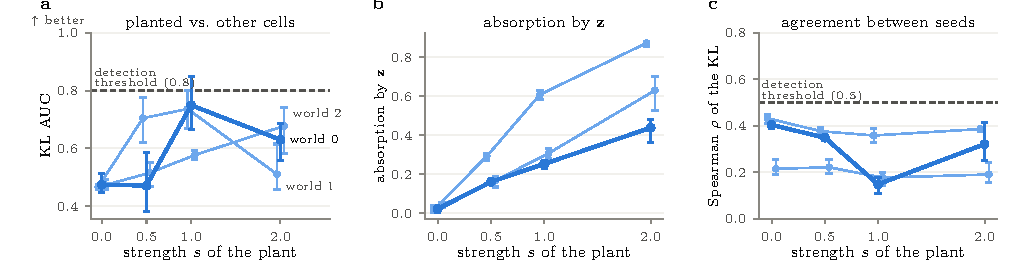
\includegraphics[width=\textwidth]{fig_planted_percell}
\caption{The planted per-cell response against its strength $s$. \textbf{a},~KL AUC separating the planted cells from the other cells of their type by their response divergence; \textbf{b},~absorption of the plant by the intrinsic latent, read through the decoder along the planted direction; \textbf{c},~the Spearman correlation of the per-cell divergence between seeds. World 0, on which the rule fixed in advance decides, in bold; worlds 1 and 2, replications, lighter. Points: mean over three model seeds (seed pairs in c); bars: their range. Dashed: the rule's detection thresholds, a KL AUC of at least $0.8$ in every seed and a Spearman correlation of at least $0.5$ in every seed pair. Arrows point toward the better direction; absorption and the agreement between seeds have none. The values are in \cref{tab:planted-percell}.}
\label{fig:planted-percell}
\end{figure*}

\input{\tablesdir/planted_percell}

\subsection{Planted Worlds}
\label{app:planted}

Three questions about the fitting procedure are answered on simulated sections, where the truth is known.

\paragraph{The amortisation gap: what is measured.}
The intrinsic encoder $q(\vz_i \mid \vx_i, t_i)$ reads a cell's counts and type but not the spill-over influx $\rhobar_i$, although the counts contain it. Its posterior mean can therefore differ from the exact posterior mean $\E[\vz_i \mid \vx_i, t_i, \rhobar_i]$ that a model told the influx would reach. This difference, the amortisation gap, cannot be measured on tissue, where the exact posterior is unknown, so we measure it on simulated sections for which the exact posterior can be computed.

\paragraph{The simulation.}
Each simulated section follows DISCELL's generative model with the response switched off, so that every quantity lies inside the model class the fit assumes and a gap measured here is a gap of inference, not of model mismatch.
\begin{itemize}
\item \emph{Cells and types.} $3{,}000$ cells at uniformly random positions in a $700\um$ square, and four types laid out in spatial patches: each cell takes the type of the nearest of twelve anchor points, three per type, up to a random perturbation, so that neighbours are often of another type and spill-over mixes types, as in tissue.
\item \emph{Intrinsic state and composition.} $\vz_i \sim \N(\mathbf{m}_{t_i}, 0.5^2\vI)$ in two dimensions, with type means $\mathbf{m}_t \sim \N(\mathbf{0}, 1.5^2\vI)$, and a clean composition $\vrho_i = \softmax(\vz_i\mathbf{A})$ over forty genes, with loadings $\mathbf{A}$ drawn from a standard normal.
\item \emph{Spill-over.} The Delaunay graph of the positions, pruned at $40\um$, with the kernel $\beta_{ij} \propto \exp(-d_{ij}/\tau)$, $\tau = 20\um$, normalised over each cell's neighbours: the model's own kernel with every face set to one. The spill-over fraction is $\kappa = 0.2$, and $\rhobar_i = \sum_j \beta_{ij}\vrho_j$.
\item \emph{Counts.} A depth $\ell_i \sim \Pois(D)$, at least $20$, for $D \in \{100, 300, 1{,}000\}$, and $\vx_i \sim \Mult\big(\ell_i, (1-\kappa)\vrho_i + \kappa\rhobar_i\big)$.
\item \emph{Image descriptor.} An eight-dimensional vector made from the cell's neighbour composition plus noise, so that the context has something to read.
\end{itemize}

\paragraph{The exact posterior.}
Given $\rhobar_i$, $\kappa$, $\mathbf{A}$, $\mathbf{m}_{t_i}$ and $\ell_i$, the posterior of $\vz_i$ is a two-dimensional density. It has no closed form, since the multinomial and the softmax are not conjugate, but in two dimensions its mean and covariance are computed to numerical precision on a $129 \times 129$ grid centred on its mode.

\paragraph{The fit and the comparison.}
DISCELL is fitted to the counts with its response channel present, as on tissue, at the final configuration (\cref{tab:architecture}) with the widths reduced to the small world ($\dz = 2$, $\dw = 2$, hidden width $128$, attention width $16$) and tiles of $512$ cells: the adversary at $\alphaa = 0.3$ with its composition term weighted three times, $\alphaw = 0.1$ with its warm-up over thirty epochs, $\alphaz = \tfrac12/\lbar$ with $\lbar$ the simulated section's median count (about $0.005$, $0.0017$ and $0.0005$ at the three depths), and the budget of $500$ epochs with patience $40$, with $15\%$ of the tiles held out for the stopping rule of \cref{sec:selection}. The posterior means are read at the accepted checkpoint. Each world is fitted at the true spill-over fraction and at spill-over fractions off by up to $0.1$ either way, with three seeds, $45$ fits in all; their accepted checkpoints lie between epochs $59$ and $434$. Because $\vz$ is identified only up to a smooth invertible map, the encoder's posterior means are first mapped onto the simulation's coordinates by a small network with five-fold cross-fitting; since the means are two-dimensional, the map cannot add information the encoder did not keep. The gap of a cell is the distance between its mapped mean and the exact mean, divided by the size of the exact posterior's standard deviation, and it is averaged over cells and over three seeds. Four references are fitted to the exact posterior mean directly, also with cross-fitting: a multilayer perceptron given the encoder's inputs, the same perceptron given $\rhobar_i$ as well, which the encoder never sees, a linear regression on the encoder's inputs, and the type mean, which knows no counts.

\paragraph{The result.}
At the true spill-over fraction the encoder's gap is $0.65$, $1.02$ and $1.93$ posterior standard deviations at the three depths (\cref{tab:planted-gap}). That is above the gap of the perceptron trained directly on the same inputs at every depth ($0.61$, $0.95$ and $1.60$), with the encoder below it in only three of the nine combinations of depth and seed, and $0.12$ to $0.58$ above the gap of the perceptron that also sees $\rhobar_i$; it is well below the linear regression's and the type mean's. The encoder's posterior mean therefore differs from the exact one by a measurable amount, more than a flexible regression on the same inputs leaves, and a regression that also sees the influx comes closer still. The gap grows with depth only in units of the posterior width, because the posterior narrows as the depth increases, from a standard deviation of $0.17$ to $0.06$; in units of $\vz$ itself it stays roughly flat, at $0.16$ to $0.17$. A wrong spill-over fraction enlarges it by a factor of at most $1.13$ over the mismatches tried, but the gap is not smallest at the true value at any depth: at $D = 1{,}000$, for instance, a spill-over fraction $0.1$ too low gives $1.77$ against $1.93$. The seed whose fits stop earliest is the worst at every depth; whether the adversary or the stopping rule accounts for the difference from the development configuration has not been tested. At that configuration (the closed-form penalty of \cref{eq:S-penalty} in place of the adversary, a fixed $600$ epochs with no stopping rule and every tile trained) the encoder's gap was smaller, $0.55$, $0.83$ and $1.48$, and below the perceptron's on the same inputs. The references are regression models of finite capacity, not information bounds, so these statements are comparative.

\begin{table}[t]
\centering
\caption{Amortisation gap on the simulated sections at the true spill-over fraction: the distance between an estimate of the posterior mean of $\vz$ and the exact one, in units of the exact posterior standard deviation, averaged over cells, mean of three seeds, by sequencing depth $D$. DISCELL is fitted at the final configuration. The DISCELL encoder is trained without the exact posterior; the other rows are fitted to it directly.}
\label{tab:planted-gap}
\small
\begin{tabular}{@{}lrrr@{}}
\toprule
& \multicolumn{3}{c}{Depth $D$} \\
\cmidrule(l){2-4}
Estimate of the posterior mean & 100 & 300 & 1{,}000 \\
\midrule
DISCELL encoder & 0.65 & 1.02 & 1.93 \\
Perceptron, the encoder's inputs & 0.61 & 0.95 & 1.60 \\
Perceptron, the encoder's inputs and $\rhobar_i$ & 0.53 & 0.80 & 1.35 \\
Linear regression, the encoder's inputs & 1.39 & 2.50 & 4.53 \\
Type mean & 2.4 & 4.1 & 7.4 \\
\bottomrule
\end{tabular}
\end{table}

\paragraph{A spill-over-subtracted encoder input.}
The intrinsic encoder could be given counts from which the expected spill-over influx has been subtracted, rather than the raw counts. On planted worlds with a known spill-over, this helped on one of three worlds. In a follow-up with twelve seeds it reversed on three of the six seeds where the comparison was not saturated, and it cost up to twenty-two points of recall of the planted signal. The encoder therefore reads raw counts, and the subtraction is kept as an option, off by default.

\paragraph{A dead response channel.}
A fit can end with a response that carries no information about the niche: the divergence of $\vw$ to its prior collapses and the context is ignored. Two checks flag it. During training, a summed divergence of $\vw$ below $10^{-5}$ over the first twenty epochs marks the fit. After training, the information between $\vw$ and the niche, on held-out cells and against a within-type permutation floor, must exceed its floor. Among the archived fits of the development period, twelve had a dead channel, nine of them on the deepest section. The KL warm-up of the final configuration removed it in every one of eight refits of that section, and the checks flag no final fit.

% S6: copied from ../aistats/appendix (see SETUP_REPORT.md for provenance); edit here, not there.
% Trimmed 2026-10-01 (agent C): cut fig:transport-heldout (same data as tab:transport-heldout), tab:moran (final values
% in main fig:programmes d; the without-adversary values kept in the text), tab:kl-summary and fig:kl-seeds (one
% paragraph keeps the negative result), and the Cellina comparison paragraph that repeats main §3.6.
\section{Results on Tissue in Full}
\label{app:full-results}

\subsection{What the Latents Carry and the Response Programmes}
\label{app:response}

\paragraph{Niche information of both latents.} With the $k$-means niches, the response carries $0.41$ to $0.63$ nats of information about the niche beyond its floor and the intrinsic state $0.06$ to $0.11$, by the nearest-neighbour estimator, over three seeds of all four sections; of the floor-corrected total, $85$ to $90\%$ lies in the response. The neural estimator agrees. These estimates use a different cell sample and floor from \cref{tab:headline-full}.

\paragraph{Hallmark labels.} \Cref{fig:hallmarks} shows the enrichment of all $50$ hallmark sets on all $34$ programmes of the twelve fits; $39$ sets are significant on at least one. EMT is significant on $30$ of the $34$ programmes, followed by oestrogen response early ($19$), KRAS signalling up ($17$), TNF$\alpha$/NF-$\kappa$B signalling and oestrogen response late ($15$ each) and coagulation ($14$); $14$ of the $39$ sets are significant on at most two programmes.

\begin{figure*}[t]
\centering
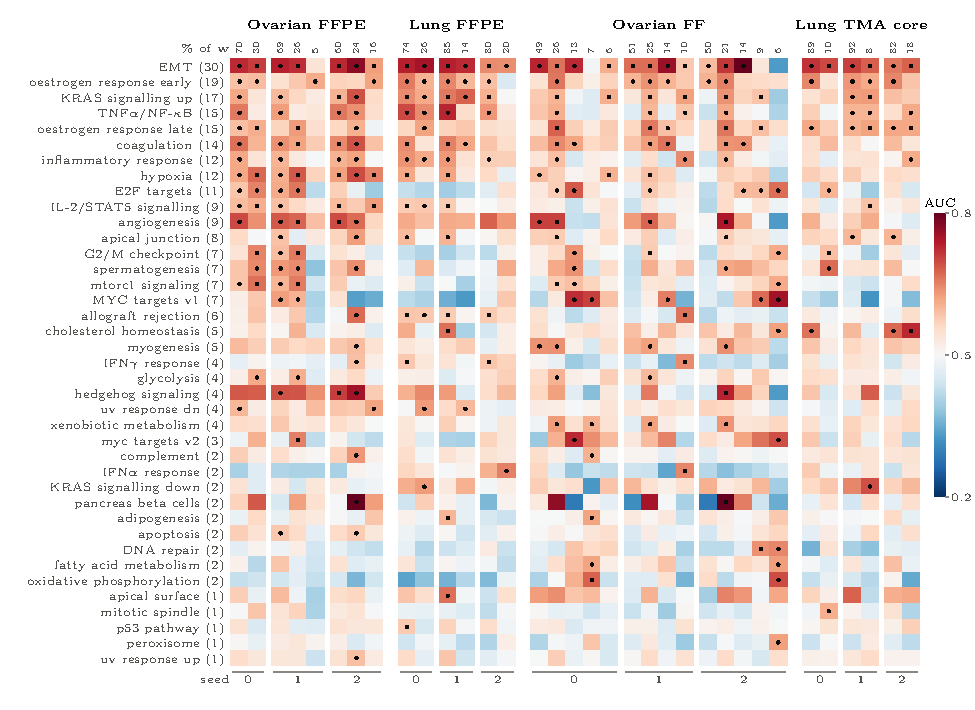
\includegraphics[width=\textwidth]{recomb_fig_hallmarks}
\caption{Hallmark labels of every response programme, by section, seed and programme (within a fit in order of variance; its share of $\vw$'s within-type variance, in $\%$, above). Rows: the sets significant on at least one programme (number of such programmes in parentheses). Cells: AUC of the Mann--Whitney test of the set's absolute loadings against the rest of the expressed panel ($0.5$ is the null); dot, $q \leq 0.05$ (Benjamini--Hochberg within each programme) with AUC above $0.5$. Programmes are identified only up to rotation, so columns are compared within a section by the recurrence of their labels, not as matched axes.}
\label{fig:hallmarks}
\end{figure*}

\paragraph{Localisation.} The first programme leans toward extracellular products (rank-biserial effect $0.08$ to $0.22$) and away from nuclear ones in every seed of the ovarian FFPE, lung and TMA sections; on the fresh-frozen section the extracellular effect is $0.17$, $0.06$ and $0.00$ in the three seeds, fading to null. A gene-specific spill-over of transcripts near the membrane would produce the same lean, and $\kappa$ carries no gene index (\cref{sec:generative}), so the lean does not distinguish a response from spill-over.

\paragraph{Signalling genes.} In the spill-over channel, ligand and receptor genes take a larger share of the between-niche shift than other genes on every section and seed (rank-biserial $0.18$ to $0.28$, $p < 10^{-13}$); in the response channel on the ovarian FFPE, lung and TMA sections ($0.12$ to $0.18$, $p < 10^{-5}$), but not on the fresh-frozen section ($0.01$ to $0.03$, $p = 0.18$ to $0.61$). MintFlow's criterion is therefore met by the spill-over channel alone on every section. The response's lean breaks down at $\kappa = 0.2$ on the fresh-frozen section (\cref{tab:kappa-star}).

\paragraph{True and false tumour axis.} On the primary section the response-predicted shifts follow the tumour bands with a mean $|\tau|$ of $0.78$ to $0.81$ and the false axis with $0.51$ to $0.56$. The contrast holds in tumour cells and macrophages and is reversed in the merged fibroblast class ($0.63$ to $0.71$ against $0.71$ to $0.75$), whose stromal half lies in deep stroma where the false coordinate follows the bands. Shifts predicted from the intrinsic state ($0.59$ to $0.65$ against $0.39$ to $0.47$), from depth ($0.57$ to $0.68$ against $0.36$ to $0.42$) and the observed shift ($0.47$ against $0.33$ to $0.36$) show contrasts of similar size: the response is closest to the bands, but the band ordering is not specific to it.

\paragraph{Marker pairs.} Exclusive double positives are $0.3$ to $2.2\%$ of held-out cells on raw counts and control double positives $1.6$ to $11.8\%$. Decoding alone lowers the exclusive rate on every section and raises the control rate on three (lowers it on the primary section), which sets the sign of this trajectory (\cref{app:sweep}). At $\kappa = 0.1$ the spill-over correction lowers both rates further (exclusive by $0.10$ to $0.50$ points, control by $0.18$ to $1.13$) and their ratio on every section, but the data show no removal specific to exclusive pairs, and the rate falls steadily with $\kappa$ with no plateau, so it does not identify the spill-over fraction.

\subsection{Without the Adversary}
\label{app:moran}

Within-type Moran's I of the posterior means (each coordinate centred on its type's mean, on the model's graph restricted to target cells, averaged with weights equal to the coordinates' within-type variance; permutation null at most $0.005$) shows what the adversary removes. Without it ($\alphaa = 0$, two seeds), I of $\vmu_z$ is $0.09$ to $0.47$; with it, $0.05$ to $0.35$ (\cref{fig:programmes}d), lower by $42$ to $48\%$ on three sections and by $25\%$ on the fresh-frozen one. What remains is within-type variation shared by neighbours that composition and the masked image do not predict (\cref{app:conditional}). Without the adversary the response's posterior mean has almost no within-type variance: summed over coordinates, below $10^{-9}$ in both fresh-frozen fits, $10^{-5}$ and $0.02$ on the ovarian FFPE section and $0.03$ to $0.12$ on the lung and TMA sections, against $3.0$ to $39$ in the final fits. The intrinsic state carries the niche instead.
% source (audit item 14): validation/validation.json morans.mu_w.var_per_dim, summed, of uncontrolledL_s0-s1 and finalL_s0-s2 (target cells, Unassigned mask); devlog 2026-09-29 "Within-type Moran's I table (results; writer)".

\subsection{The Response at the Type Level}
\label{app:kl-maps}

The per-cell divergence of the response from its prior is small, $0.004$ to $0.09$ nats per cell, and differs up to ten-fold between seeds. Within one fit it is spatially organised (Moran's I $0.15$ to $0.85$), but which cells deviate does not reproduce between seeds (per-cell rank correlation $-0.43$ to $0.57$). Under a rule fixed in advance (odds ratio at least $1.5$ or standardised difference at least $0.3$, interval clear of the null, in all three seeds), the top decile differs from the other cells only coarsely: it avoids tumour on the two FFPE sections and lies among fibroblasts (ovarian) and chondrocytes (TMA core); nothing passes on the fresh-frozen section and no continuous feature passes anywhere. The divergence is therefore not a per-cell anomaly score at the operating point, and a planted per-cell response is not detected at this weight either (\cref{app:planted-percell}). The posterior standard deviation of $\vw$ is $0.98$ to $1.01$: the response posterior is its prior in spread as well as in location. The intrinsic state's divergence and standard deviation do reproduce between seeds (rank correlations $0.78$ to $0.93$ and $0.53$ to $0.93$); deeper cells have smaller divergences and wider posteriors (pooled $\rho = -0.77$ to $-0.39$ and $0.21$ to $0.73$), the per-cell scaling of \cref{app:pathb}. The intrinsic state is thus regularised less in low-count cells, and a deep cell's posterior width overstates its uncertainty, one more reason the reported uncertainty comes from the sweep and the seeds rather than from $q$.

\subsection{Relocation in Full}
\label{app:cellina-cf}

\paragraph{Against Cellina.} Cellina's neighbour-rewiring counterfactual \citep{moeed2026cellina} is refitted on the training tiles only, decoded at its posterior mean, and scored by our relocation reads on the panels, niches, ceilings and bootstrap draws of DISCELL's first seed (\cref{tab:cellina-cf}). It has no spill-over channel, so its prediction cannot be split into programme and spill-over parts. The comparison is of one Cellina fit with one DISCELL seed; main \cref{tab:relocation} reads it.

\input{\tablesdir/cellina_cf}

\paragraph{On held-out tiles.} The relocation read is cross-fitted over spatial folds drawn from every tile, so most of its scored cells lie in the model's training tiles. \Cref{tab:transport-heldout} scores the same read on held-out tiles only, with every model quantity still estimated from training tiles and the same panels, ceilings and mask. The rule set before the read was to reconsider the cross-fitted read if the held-out fraction of the ceiling fell outside its interval on any section; it did, in both directions, and the cross-fitted read was kept, because an in-sample advantage would lower the held-out read throughout and the fraction of the ceiling does not move that way. The single-cell read does, on $11$ of $12$ fits. The held-out pool is about three quarters of the cross-fitted one, so fewer panels reach the trusted tier and several all-panel fractions exceed one; on the TMA core no panel is trusted on held-out tiles. On held-out tiles Cellina's fraction of the ceiling stays above DISCELL's range on the ovarian FFPE section and falls below it on the lung section.

\input{\tablesdir/transport_heldout}

\paragraph{Against a plain regression.} On the panels of each seed's relocation read, a ridge regression of the type's expression on its neighbour composition is fitted to the raw counts of the cells that supply the model quantities, and its predicted shift between the two niches is scored by the same fraction of the ceiling. Fitted on $\log(1+x)$ at the median depth, as first specified, it recovers $0.06$ to $0.22$ of the ceiling in the trusted tier; fitted on depth-normalised rates, the scale of the read, it recovers $0.81$ to $0.89$ on the three whole-slide sections (DISCELL $0.65$ to $0.72$) and $0.77$ on the TMA core (DISCELL $0.73$, two seeds with a trusted panel). Over all panels DISCELL is higher on the TMA core and the two FFPE sections, and lower on the FF section ($0.66$ against $0.79$). The single-cell read cannot score the regression against DISCELL's decode of the target cells, so both are scored against the raw target cells: the gap closed is $0.48$ to $0.62$ for the regression and $0.25$ to $0.63$ for DISCELL. Because the observed shifts contain the spill-over, none of these reads can favour a model for separating it (\cref{sec:relocation}); in simulation, scored against the spill-free shift, they can (\cref{app:S-reloc-clean}).
% Source: scripts/logs/recomb_additions_2026-10-01/READOUT.md (3-seed means over finalL_s0-s2; per seed in
%   data/datasets/<ds>/experiments/transport_regression_reference.md). Deviation 2 and 3 of the devlog launch entry.

\subsection{The Latents on Every Section}
\label{app:latents}

\Cref{fig:latents-umap} extends main \cref{fig:latents-main} to all four sections. The type of panels c and d is chosen by a rule: among types with at least $3{,}000$ cells, the one whose neighbourhoods are most mixed. UMAP distorts distances, so the figure illustrates what the probe (\cref{tab:probe}) measures and replaces it nowhere.

\begin{figure}[tp]
\centering
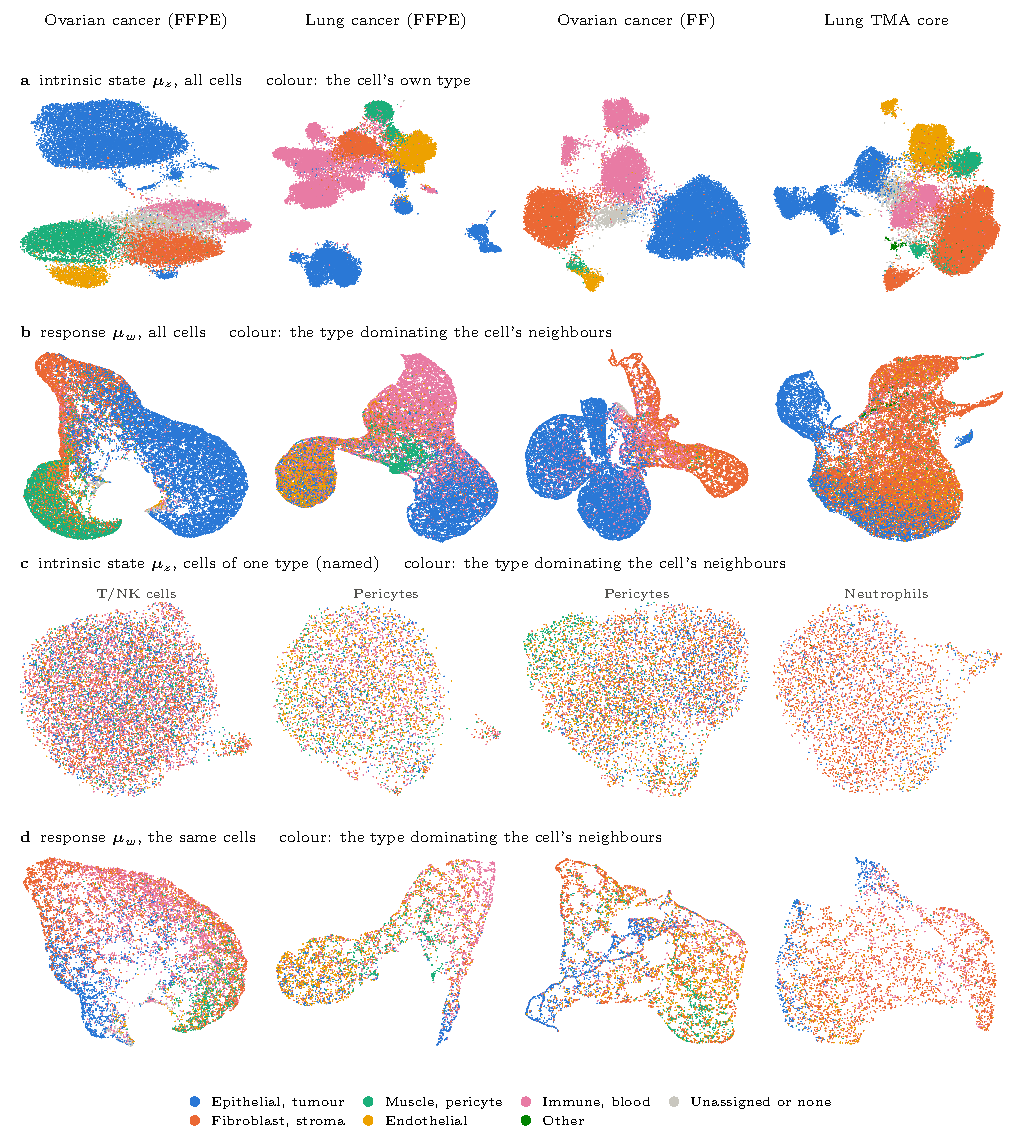
\includegraphics[width=0.8\textwidth]{fig_latents_umap}
\caption{UMAP of the posterior means, one seed of the final configuration; columns: the four sections. \textbf{a},~$\vmu_z$ of $30{,}000$ random cells, coloured by the cell's lineage family. \textbf{b},~$\vmu_w$ of the same cells, coloured by the family dominating its graph neighbours (grey if none). \textbf{c},~$\vmu_z$ of up to $10{,}000$ cells of one type (named above), coloured as in b. \textbf{d},~$\vmu_w$ of the same cells. Families as in \cref{fig:sections}.}
\label{fig:latents-umap}
\end{figure}

\subsection{Training Cost}
\label{app:timing}

\Cref{tab:timing} gives the cost of a fit. DISCELL's time per epoch is pure training; its wall-clock time covers the three final fits including evaluations every five epochs and the early stop, whereas the comparison methods' times are training only, as recorded for the fits compared here. MintFlow's whole-section fits took $14.8$ (lung FFPE) and $15.8$ hours (ovarian FFPE) of wall-clock time, against $3.2$ to $7.4$ minutes for a whole DISCELL fit of the lung section; the other whole-section SIMVI and MintFlow fits could not be run (reasons in \cref{tab:baselines,tab:timing}). The cost of an epoch is linear in the number of cells, and peak memory is the resident count matrix plus the spill-over influx over the edges of a tile, which the tile size bounds (\cref{app:tiles}). The sweep costs eighteen fits per section. Sample size is not analysed beyond the range of sizes in \cref{tab:sections}.

\input{\tablesdir/timing}

% S8 (rendered as S7 after the reorder): copied from ../aistats/appendix (see SETUP_REPORT.md for provenance); edit here, not there.
% Trimmed 2026-10-01 (agent D): tab:breakdown (duplicate of main tab:kappa-star), tab:kappa-sweep (same values as
% fig:kappa-sweep) and fig:sensitivity (same values as tab:sensitivity) cut; tab:breakdown-traj is the generated
% compact table breakdown_traj_main.tex (means of four trajectory readouts plus the probe re-graded across the sweep).
\section{Spill-over Sweep and Sensitivity}
\label{app:sensitivity-section}

\subsection{The Claimed Contrasts and the Rules}
\label{app:sweep}

\Cref{tab:S-contrasts} defines the contrasts whose breakdown points the main text reports (\cref{tab:kappa-star}), and \cref{fig:breakdown-data} draws them across the grid. Two contrasts first in the graded set were moved to trajectories after reading (\cref{tab:breakdown-traj}): the marker-pair contrast, which measures the decode rather than the spill-over correction, being already present at $\kappa = 0$, and the relocation's margin over its programme part, which is zero at $\kappa = 0$ by construction. A section's set holds seven contrasts on each whole-slide section and six on the TMA core and on its serial section, which have no tumour cells for the tumour axis.

\emph{Rules.} No readout was designated primary in advance: the final sweeps were preceded by development sweeps, so any such set would have been chosen with knowledge of earlier results. The interval of a contrast is for its mean over seeds, from a spatial block bootstrap over tiles within each seed's fit, two-sided and Bonferroni-adjusted over the claimed contrasts of the section; rankings are read through pairwise differences, each with its own breakdown point. Findings are section-level. A tissue-specific finding is claimed only if it holds on both serial sections of a tissue where two exist. Only the TMA core has one, and every contrast of the core's set is read on it through the core's fits. Each replicates the core's finding, except the relocation's margin over its spill-over part, which holds on the core over the whole grid and on the serial section only up to $\kappa = 0.3$; on the TMA, that finding is therefore claimed up to $\kappa = 0.3$. A property of the method, such as whether a readout moves with $\kappa$ at all, is required on every section. A decline along the grid is mechanical, since a larger $\kappa$ assigns more of the neighbours' resemblance to the mixture; a change in the direction of a programme or in which latent a target aligns with is not. Programmes are identified only up to rotation and per-column constants (\cref{app:symmetries}), so raw loadings and probe directions are never compared across runs. The interval at a grid point is a sampling statement that narrows with more cells; the trajectory across the grid is not, because the confound it expresses is not a sampling problem.

% Formulas from S5 (app:readouts) and scripts/logs/breakdown_2026-09-29/FAMILY.md ("Members"); names as in main tab:kappa-star.
\begin{table}[!htbp]
\centering
\caption{The claimed contrasts, named as in \cref{tab:kappa-star}. Each is signed so that a finding is positive; its breakdown point follows \cref{def:breakdown}. The relocation reads are defined in \cref{app:readouts}, the signalling share and the tumour axis in \cref{app:readouts} and \cref{app:response}. The tumour axis needs tumour cells to define the bands, so it is not read on the TMA sections; the serial section is read through the core's fits. Which contrasts are read on which section follows \cref{tab:kappa-star}.}
\label{tab:S-contrasts}
\footnotesize
\setlength{\tabcolsep}{3pt}
\begin{tabular}{@{}p{0.2\textwidth}p{0.4\textwidth}p{0.28\textwidth}c@{}}
\toprule
Contrast & Definition & Positive means & Main text \\
\midrule
\multicolumn{4}{@{}l}{\emph{Biological claims}} \\
\TermReloc{} $>$ \termSpill{} part & mean $R^2$ over all panels of the prediction with programmes and spill-over, minus that of the spill-over part alone & the programmes add to what spill-over predicts & \cref{sec:relocation} \\
\TermReloc{} $>$ type mean & median over panels of the gap closed by the relocated cells (single-cell read), minus that closed by copies of the target's mean profile (type-mean reference) & moved cells match the target's distribution, not only its mean & \cref{sec:relocation} \\
Nearest-twin advantage & median over panels of $(d_{\text{random}} - d_{\text{twin}})/d_{\text{random}}$, Hellinger distances from a target cell to its nearest relocated cell in $\vmu_z$ and to a random one (twin read) & the intrinsic state picks the right counterpart & \cref{sec:relocation} \\
Signalling-gene lean of $\vw$ & rank-biserial effect of the per-gene response share, ligand and receptor genes against the other genes & signalling genes take more of the response & \cref{sec:results-sweep} \\
Tumour axis in $\vw$ & mean $|\tau|$ of the response-predicted shift with the tumour-proximity bands, minus that with a false spatial axis & the response follows the bands & \cref{sec:results-sweep} \\
\addlinespace
\multicolumn{4}{@{}l}{\emph{Allocation checks}} \\
Cycle in $\vz$, not in $\vw$ & cycle $R^2$ of $\vmu_z$ minus that of $\vmu_w$, top-decile cycling held-out cells, centred per type & the cycle is in the intrinsic state & \cref{sec:results-z} \\
Niche information in $\vw$ & $\I(\text{niche}; \vmu_w)$ minus its within-type permutation floor, held-out cells, nats & the response carries the niche beyond the type & \cref{sec:results-w} \\
\bottomrule
\end{tabular}
\end{table}

\begin{figure}[!htbp]
\centering
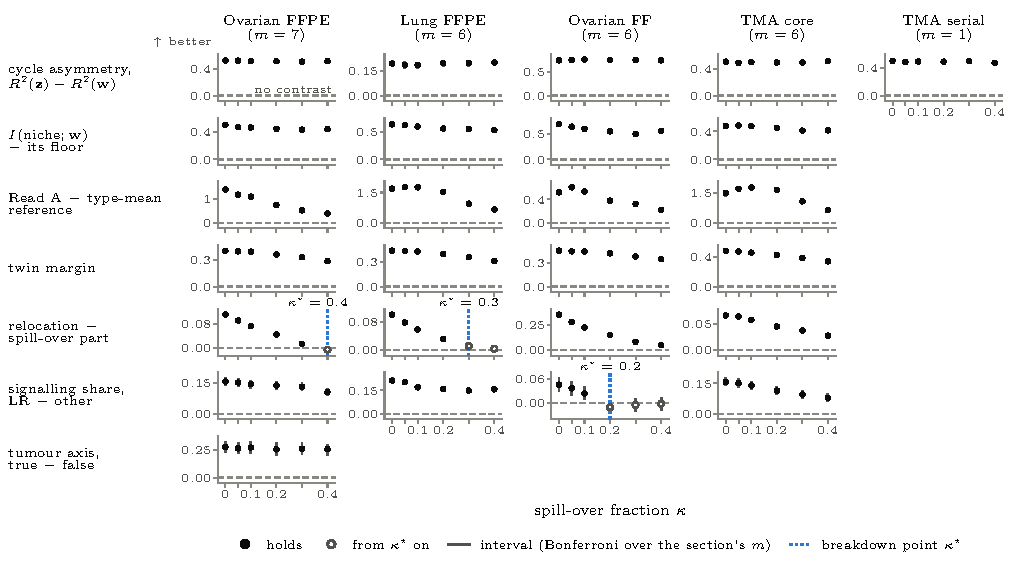
\includegraphics[width=\textwidth]{recomb_fig_breakdown_data}
\caption{The claimed contrasts (\cref{tab:S-contrasts}) across the spill-over sweep; $m$, the number of contrasts in the section's set. At each $\kappa$, the mean over three seeds and its Bonferroni-adjusted interval; filled: the contrast holds; hollow: from $\kappa^\star$ on (dotted). Each panel has its own vertical scale, which includes zero (dashed); empty panel: not in that section's set.}
\label{fig:breakdown-data}
\end{figure}

Every contrast holds across the grid, on every section where it is read, except in six cells over three contrasts: the tumour axis, which breaks down at $\kappa = 0.4$ on the lung section and $0.3$ on the fresh-frozen section; the signalling-gene lean on the fresh-frozen section, at $0.2$; and the relocation's margin over its spill-over part, at $0.4$ on the primary section, $0.3$ on the lung section and $0.4$ on the serial section. All but the signalling-gene lean break because a seed changes sign.

\subsection{Diagnostics and Trajectories across the Sweep}

\Cref{fig:kappa-sweep} draws the diagnostics of every fit of the sweep, and \cref{tab:breakdown-traj} the readouts reported as trajectories: magnitudes, positive under any fit, and the two reclassified contrasts. The relocation's margin over its programme part is positive in every seed on every section from $\kappa = 0.05$ to $0.2$; it stays positive up to $\kappa = 0.4$ on the lung and fresh-frozen sections and turns negative on the primary section from $\kappa = 0.3$ and, in the mean, on the TMA core at $0.4$. The relocation read's fraction of the ceiling is lower at $\kappa = 0$ than at the operating point on every section, peaks at $\kappa = 0.05$ to $0.2$ and falls beyond, most on the primary section, where it reaches $0.35$ at $\kappa = 0.4$. As $\kappa$ grows, Moran's I of the intrinsic state falls on every section, while that of the response changes by at most $0.05$. The within-type share of the response's variance ($0.26$ to $0.31$ on the primary section, $0.40$ to $0.44$ on the lung section, $0.53$ to $0.56$ on the fresh-frozen section, $0.49$ to $0.55$ on the TMA core) and the effective number of programmes (at most one axis apart on a section) change little, and the overlap of the programme spaces with the reference fit stays at $0.76$ to $0.92$ on average, comparable to the overlap between seeds at the operating point (lowest member $0.72$ to $0.84$), with a mild decline at $\kappa = 0.4$.
% within-type share, effective rank, Moran's I of mu_w and programme overlap: generated breakdown_traj.tex (tab:breakdown-traj), means over seeds.

The held-out probe is graded at every grid point. The nonlinear probe's composition residual, as a seed mean, is $4.0$ to $4.7\%$ on every section from $\kappa = 0$ to $0.1$ and $2.9$ to $4.5\%$ beyond, with single seeds between $2.0$ and $6.1\%$ over the whole grid (\cref{tab:breakdown-traj}). The invariance therefore does not weaken along the grid, and a readout's change with $\kappa$ is not a change in the residual niche signal.
% source: data/datasets/{xenium_prime_ovarian_cancer_ffpe,xenium_prime_human_lung_cancer_ffpe,xenium_prime_human_ovary_ff,gse315411_pdltma06_11_prime_solo}/experiments/probe_regrade_lineage_sweep.json,
%   key mlp_comp.excess per run, shown as 1 - exp(-2 excess) as in tab:probe (the kappa = 0.1 rows reproduce tab:probe's 4.0-5.5, 4.2-5.0, 4.4-5.0, 3.5-4.8).

\begin{figure*}[!htbp]
\centering
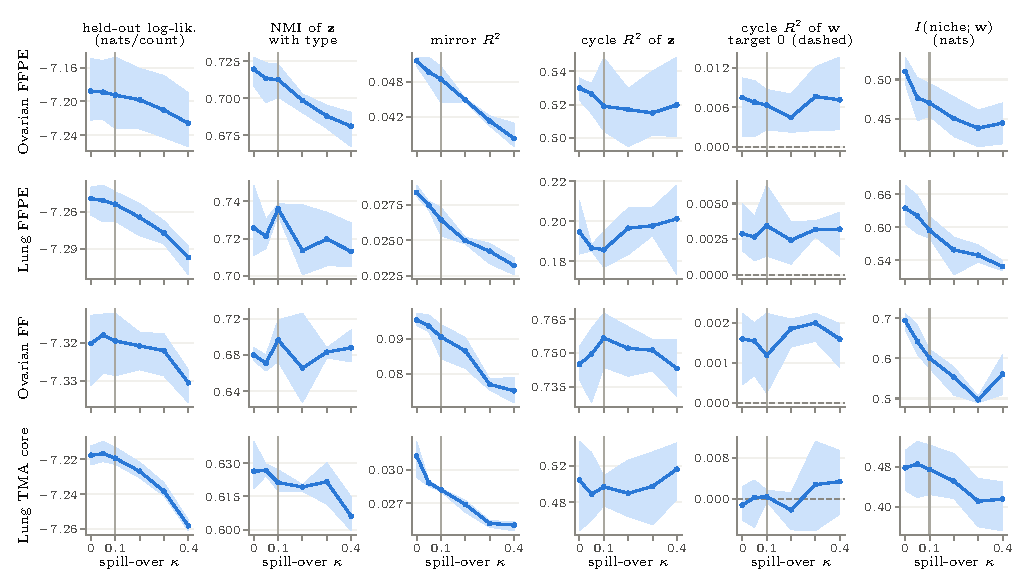
\includegraphics[width=\textwidth]{recomb_fig_kappa_sweep}
\caption{The diagnostics across the spill-over sweep, per section: held-out reconstruction (nats per count), NMI of $\vz$ with the type, mirror $R^2$, cycle $R^2$ of $\vz$ and of $\vw$ (expected near zero, dashed) on the top-decile cycling set, and $\I(\text{niche}; \vw)$ above its within-type floor (nats). Line: mean over three seeds; band: their range; vertical line: the operating point $\kappa = 0.1$. These readouts move with $\kappa$ by construction, and $\kappa$ is not selected on them: $\kappa = 0.1$ matches the typical per-cell misassignment \citep{yang2025mistic}.}
\label{fig:kappa-sweep}
\end{figure*}

\input{\tablesdir/breakdown_traj_main}

\subsection{A Planted Spill-over Control}
\label{app:S-planted-spillover}

In simulation, a spatial contrast made only by spill-over at a known fraction $\kappa_{\text{true}}$ is planted beside a genuine response contrast, and the sweep is run with the rule of \cref{sec:results-sweep} (\cref{tab:S-planted-spillover}). The world has $30{,}000$ cells of eight types and $60$ genes, $20$ of which carry spill-over but no planted response; it is fitted at the final configuration, three seeds at every grid point, for $\kappa_{\text{true}} = 0$, $0.1$ and $0.2$. The prediction, set before the run, was that the contrast made by spill-over breaks at the first grid point at or above $\kappa_{\text{true}}$ and the genuine contrast holds over the grid.

The contrast as first defined, the $R^2$ gain of the full prediction over its spill-over part on the genes without a response, was mis-specified: its programme term enters with a penalty that is never positive, so it cannot vanish at $\kappa = 0$ and is a finding even in the world without spill-over. A diagnostic on the same fits traced this to the definition, not to the simulator or to spill-over, and the contrast was corrected to the programmes' alignment with the part of the observed shift that the clean shift does not explain, which is zero in expectation when nothing spills over. Both are reported.

The corrected contrast is no finding without spill-over and breaks at $\kappa^\star = 0.05$ and $0.1$ when $0.1$ and $0.2$ are planted: ordered as the planted fractions, and one grid step earlier than predicted, so it is flagged conservatively; its point estimate changes sign between $\kappa_{\text{true}}$ and the next grid point in both worlds. The genuine response contrast holds over the whole grid without spill-over and through $\kappa = 0.2$ when spill-over is planted ($\kappa^\star = 0.3$), in both worlds beyond the spill-over contrast. The breakdown points thus order a contrast made by spill-over below a genuine one; they do not recover $\kappa_{\text{true}}$, as \cref{def:breakdown} says. The intervals are wide, and the programmes fit a little of the count noise of the scored cells that lie in their training tiles, which keeps the corrected contrast's point estimates above zero in the null world.

\input{\tablesdir/planted_spillover}

\subsection{Relocation against the Spill-free Shift}
\label{app:S-reloc-clean}

On tissue, relocation is scored against observed shifts, which contain the spill-over (\cref{sec:relocation}). On the planted worlds of \cref{app:S-planted-spillover} the simulator also knows the clean shift between niches, without spill-over and count noise, on the same panels (\cref{tab:S-reloc-clean}). The prediction, set before the read, was that the regression degrades against the clean shift as $\kappa_{\text{true}}$ grows, and DISCELL less. It holds for DISCELL's spill-free part: the prediction from the programmes alone explains $R^2 = 0.76$ of the clean shift at every planted fraction, about $0.88$ of its noise ceiling, and $0.73$ at the operating point when $0.2$ is planted, while the regression falls from $0.40$ to $0.14$ on the log scale and below zero on the rate scale. It does not hold for DISCELL's full prediction, which adds the predicted spill-over and so, by design, targets the observed shift; against the clean shift it degrades as the regression does. Against the observed shift, as on tissue, the full prediction and the rate-scale regression are level whenever spill-over is planted. The worlds are drawn from DISCELL's own generative model, so this shows that the separation recovers the spill-free shift when the model's form of spill-over holds, not that it does on tissue.

\input{\tablesdir/reloc_clean}

\subsection{Sensitivity to the Assumptions}
\label{app:sensitivity}

\input{\tablesdir/sensitivity}

\Cref{tab:sensitivity} refits the final configuration with one setting changed at a time, on the primary section and, for two of the families, on the TMA core and the fresh-frozen section, and gives each arm's move in units of the final configuration's standard deviation over its three seeds. An arm has two or three seeds, and that standard deviation is itself a rough estimate, so moves of one or two units are within what a change of seed can produce. Nothing is adopted from these arms.

\paragraph{The form of the spill-over.} The rate is set per cell, in proportion to the ratio of its neighbours' depth, or density, to its own (capped), or per gene, in proportion to the gene's share of transcripts detected outside nuclei, each at the same mean rate as the section-wide $\kappa$. No read moves by more than $1.3$ standard deviations, and the relocation read stays at $0.65$ to $0.66$. Forms outside these three are not tested.

\paragraph{A false-positive floor.} The model has no background term (\cref{app:limitations}). A fixed floor added to the mixture, one rate per section or one per cell scaled by its area, leaves every diagnostic of the primary section within $0.6$ standard deviations, but lowers its relocation read from $0.65$ to $0.50$ ($-8.3$) with the per-section floor and to $0.54$ ($-6.2$) with the area-scaled one, the largest moves in the table. On the TMA core the floor leaves the relocation read at $0.73$ and moves the agreement with type up by $2.4$ and the mirror down by $4.0$ standard deviations of a very narrow spread. The relocation read on the primary section therefore depends on the absence of a background term, and it is the read to treat with most caution there.

\paragraph{The response weight.} The operating point $\alphaw = 0.1$ lies far above the bound-equivalent value $1/\lbar$ (\cref{app:pathb}): $\alphaw = m/\lbar$ with $m$ of about $14$ on the primary section, $28$ on the TMA core and $143$ on the fresh-frozen section. Lowering it opens the per-cell channel: at $\alphaw = 1/\lbar$ the response's deviation from its prior mean carries $3.5\%$ of its variance on the primary section and $21\%$ on the TMA core, against $0.2\%$ at the operating point, and adds $0.015$ to $0.017$ nats per count to held-out reconstruction, against at most $0.001$. The cost is in the agreement of $\vz$ with type, which falls by $2.6$ and $2.8$ standard deviations ($0.684$ against $0.713$, $0.607$ against $0.621$), and by $2.9$ on the fresh-frozen section at $10/\lbar$ ($0.629$ against $0.697$). The lower weights raise the relocation read on the primary section ($0.71$ at $1/\lbar$) and on the fresh-frozen section ($0.75$ at $5/\lbar$ and $10/\lbar$), but not on the TMA core. The operating point thus keeps the agreement with type at the price of a closed per-cell channel (\cref{app:planted-percell}). The deviation's share of variance and its held-out gain come from the same fits but are not in the table.

\paragraph{The adversary.} Doubling the heads' update steps or their width, or averaging an ensemble of three heads, changes the nonlinear composition residual by at most $0.7$ standard deviations; doubling the steps costs $4.3$ in agreement with type. Weighting the composition term equally with the image term instead of three times raises the residual from $4.6\%$ to $6.6\%$ ($+2.5$) and the mirror by $2.0$; a weight of five lowers the residual to $3.7\%$ at a cost of $2.1$ in agreement with type.

\paragraph{Without the intrinsic path.} The final configuration is refitted on all four sections with $\omega = 0$, three seeds at the final fits' splits. The prediction, set before the fits: the allocation shifts toward $\vw$, so the agreement of $\vz$ with type and its cycle $R^2$ fall, those of $\vmu_w$ rise, and the within-type share of $\vw$'s variance changes. A read counts as moved when the mean over seeds lies outside the final fits' range. Two reads move on every section with disjoint ranges: the NMI of $\vmu_w$ with the type rises ($0.42$ to $0.50$ on the primary section, $0.27$ to $0.32$ on the lung section, $0.33$ to $0.35$ on the fresh-frozen section, $0.29$ to $0.40$ on the TMA core), and the within-type share of $\vw$'s variance falls ($0.32$ to $0.19$, $0.43$ to $0.37$, $0.53$ to $0.49$, $0.53$ to $0.33$). The intrinsic state loses less: its cycle $R^2$ falls on the fresh-frozen section ($0.76$ to $0.70$, disjoint ranges); on the primary section its agreement with type ($0.71$ to $0.67$) and cycle $R^2$ ($0.52$ to $0.50$) fall by the mean only; elsewhere both stay within range. The cycle $R^2$ of $\vw$ rises nowhere, no read without a prediction moves with disjoint ranges, and no move is opposite to the prediction. The path's role is thus to keep the type out of $\vw$. One final fit on the TMA core, refitted with the software used for the ablation, comes out close to but not identical to the original (NMI of $\vz$ $0.616$ against $0.621$, just below the final fits' range); the moves above are larger.


\subsection{What Each Part of the Model Buys in Reconstruction}
\label{app:recon-modes}

\begin{table}[!htbp]
\centering
\caption{Held-out reconstruction by what the decode may use, in nats per count: mean over three seeds, with the range. \emph{Full}: log-likelihood per count of the full decode, mean only. The other columns are differences: context over type profile, intrinsic over context (the cell's own $\vz$), full over intrinsic (the cell's own $\vw$). Every difference has a $200\um$ tile-bootstrap $95\%$ interval; all exclude zero except context over type profile on the lung FFPE section, and on the TMA core for one seed. Target cells of held-out tiles; for the serial section, every cell, read through the model fitted to the core.}
\label{tab:recon-modes}
\small
\setlength{\tabcolsep}{4pt}
\begin{tabular}{@{}lcccc@{}}
\toprule
Section & Full & Context & Own $\vz$ & Own $\vw$ \\
\midrule
Ovarian cancer (FFPE) & $-7.19$ & 0.025 (0.019--0.029) & 0.133 (0.116--0.154) & 0.0008 (0.0008--0.0010) \\
Lung cancer (FFPE) & $-7.25$ & $-0.000$ ($-0.001$ to $0.000$) & 0.167 (0.163--0.171) & 0.0004 (0.0003--0.0005) \\
Ovarian cancer (FF) & $-7.32$ & 0.033 (0.032--0.034) & 0.059 (0.057--0.061) & 0.0001 (0.0001--0.0001) \\
Lung TMA core & $-7.22$ & 0.007 (0.003--0.013) & 0.127 (0.124--0.129) & 0.0004 (0.0003--0.0005) \\
Lung TMA, serial section & $-7.24$ & 0.010 (0.008--0.012) & 0.127 (0.125--0.129) & 0.0004 (0.0003--0.0005) \\
\bottomrule
\end{tabular}
\end{table}

Held-out reconstruction reads a cell's counts twice, in the encoder and in the likelihood, so one number of it says little. \Cref{tab:recon-modes} decodes the held-out cells in four ways: the \emph{type profile} (the type's empirical count profile); the \emph{context} decode, which uses none of the cell's counts ($\vz$ at its type's mean, $\vw$ at the prior mean $\mpsi(\vc_i, t_i)$); the \emph{intrinsic} decode (own $\vz$, $\vw$ at the prior mean); and the \emph{full} decode. The spill-over influx and $\kappa$ are the fit's in every decode. The cell's own intrinsic state carries most of what the model adds over the type profile; the context adds a little on three sections and nothing on the lung FFPE section; the response's own posterior adds one part in a thousand or less beyond its prior mean, by the operating point's design (\cref{app:pathb}), with the lung section the exception on subtype recovery (\cref{app:subtype}). The model fitted to the TMA core reads its serial section as it reads the core.


% S9 (rendered as S8 after the reorder): copied from ../aistats/appendix (see SETUP_REPORT.md for provenance); edit here, not there.
\section{Limitations}
\label{app:limitations}

The conclusion names the main limitations; this section collects them all, each with where it is argued.
\begin{itemize}[leftmargin=*,itemsep=2pt]
\item \emph{The form of the spill-over.} One fraction per section, the same for every gene, scaled by the receiving cell's own rate, and no ambient term (\cref{sec:generative}). A low-count cell beside high-count donors is therefore under-corrected at every $\kappa$ and the reverse over-corrected; the niche-predictable part of that error lands in $\vw$, and the sweep does not address it. Ambient RNA captured by the panel's own probes is not registered by the negative controls \citep{janesick2023} and is not modelled. If extranuclear transcripts, enriched for secreted and membrane proteins \citep{xia2019merfish}, cross boundaries more readily, that gene-specific spill-over is spanned by no $\kappa$ and lands in $\vw$, so a programme enriched for cell-surface genes cannot be separated from it by the sweep. Three other forms move no read on the primary section by more than $1.3$ seed standard deviations, but a fixed false-positive floor lowers the relocation read from $0.65$ to $0.50$ (\cref{app:sensitivity}).
\item \emph{What the sweep separates.} Spill-over of the modelled form from a spatial association, not spatially organised intrinsic variation within a type, which the conditional invariance assigns to the response, nor cells selecting their niche (\cref{sec:sweep}). The bound of \cref{prop:kappa-bound} holds with the neighbours' clean profiles fixed and is not computed on any section, so the grid supports only survival up to $\kappa = 0.4$.
\item \emph{Labels.} The labels come from the same counts, spill-over included, and the decomposition is relative to their granularity: a spatially clustered state merged into its lineage, such as a subclone, is read as a response (\cref{app:conditional}). Label errors caused by spill-over concentrate at heterotypic interfaces and in low-count cells, and enter through $t_i$ and the neighbours' compositions, where neither $\kappa$ nor the invariance reaches them.
\item \emph{The invariance is incomplete.} A nonlinear probe still recovers $3.5$ to $5.5\%$ of the within-type variance of neighbour composition from $\vz$ on every section, and on the TMA core the adversary removes only $29$ to $48\%$ of what the model without it leaves (\cref{tab:probe}). The development threshold, a quarter of the uncontrolled excess, is not met on composition on three sections and on the image block on the TMA core, so the residual is reported descriptively. A probe at its floor bounds only the dependence it can detect.
\item \emph{The response at the operating point.} With $\alphaw$ far above its bound-equivalent value, the response readouts are in effect readouts of the context regression; the lung section is a partial exception (\cref{app:subtype}). The per-cell channel is closed by design, not by the data: a planted per-cell response is not detected and is partly absorbed by $\vz$ (\cref{app:planted-percell}), and lowering $\alphaw$ opens the channel at a cost in agreement with type (\cref{app:sensitivity}). Several response readouts are not specific to it: the ligand--receptor criterion is met by the spill-over channel alone, the lean toward membrane and secreted genes is what gene-specific spill-over would produce, and the tumour band ordering is also followed by $\vz$ and by depth (\cref{app:response}).
\item \emph{The cycle reference.} The cycle scores are gene-set scores of the cell's own segmented counts, into which spilled-over transcripts and environment-induced expression enter; the asymmetry between the latents shows where the model places this axis, not that it is the cell's own (\cref{sec:results-z}).
\item \emph{Inference.} The intrinsic encoder does not see the spill-over influx; in simulation its posterior mean is $0.65$ to $1.93$ posterior standard deviations from the exact one, more at every depth than a perceptron fitted on the same inputs, and on tissue the gap cannot be measured (\cref{app:planted}). The objective is a weighted surrogate, so the uncertainty reported comes from the sweep and the seeds, not from the posterior (\cref{app:pathb}); it is not unimodal in the seed, and fits with a dead response channel were discarded and re-seeded (none among the final fits).
\item \emph{Identification.} Beyond the upper bound on $\kappa$ and the invariance the probe grades, nothing guarantees that the intrinsic and response coordinates are identified (\cref{sec:sweep}).
\item \emph{Evaluation.} Cells of held-out tiles enter training as stop-gradient neighbours (\cref{app:tiles}). Every fit is to one section of one platform, only one section is held out whole, and sample size is not analysed. Most cells scored by the relocation reads lie in training tiles; on held-out tiles the fraction of the ceiling moves both ways and the single-cell read falls (\cref{tab:transport-heldout}). Relocation is scored against observed shifts, which contain the spill-over, and a plain regression on the raw counts reproduces them as well or better (\cref{app:cellina-cf}); on tissue it shows that the whole model works, not that the separation is right, which is checked against the spill-free shift only in simulation from the model's own generative process (\cref{app:S-reloc-clean}). The comparison methods ran at their published defaults on our held-out cells, while DISCELL's weights were calibrated on these sections (\cref{sec:setup}); two could not be run on some sections (\cref{tab:baselines}). Edge features in the attention were not tested.
\end{itemize}

\FloatBarrier

\bibliographystyle{unsrtnat}
\bibliography{../aistats/references}

\end{document}
